% TODO
% Deben incluir los resultados de los experimentos, utilizando el formato mas adecuado
% para  su  presentacion.   Deberan  especicar  claramente  a  que  experiencia  corresponde
% cada resultado.  No se incluiran aqu corridas de maquina.
\subsection{Performance}
\subsubsection{Performance de los m\'etodos en funci\'on de la discretizaci\'on para una instancia}
Utilizamos una heur\'istica para poder determinar mejor el orden c\'ubico de la curva resultado. Sea $f(x)$ el valor del tiempo de c\'omputo, graficar $f(x)/x^k$, siendo $k \in \left[ 2, 3, 4 \right] $ . De ser $f(x)$ de orden c\'ubico, esperar\'iamos que para el polinomio de orden 2 el resultado sea una funci\'on creciente, para el de orden 3 el resultado se asemeje a una constante y para el de orden 4, una funcion decreciente.

\begin{center}
\textbf{1 instancia por archivo de test}\\
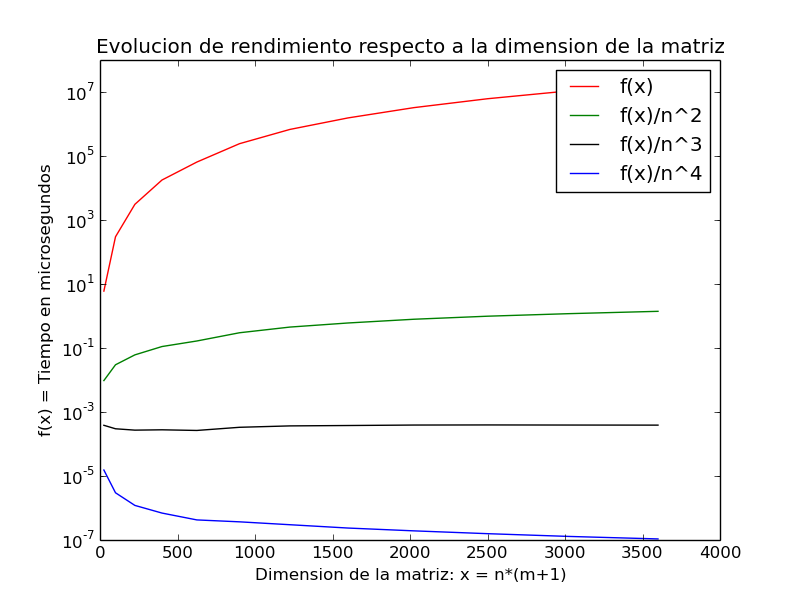
\includegraphics[scale=0.35]{experimentos2a_2b/tiempos_nm_fitteo_1_inst/eliminacion_gaussiana_time_consumed.png}
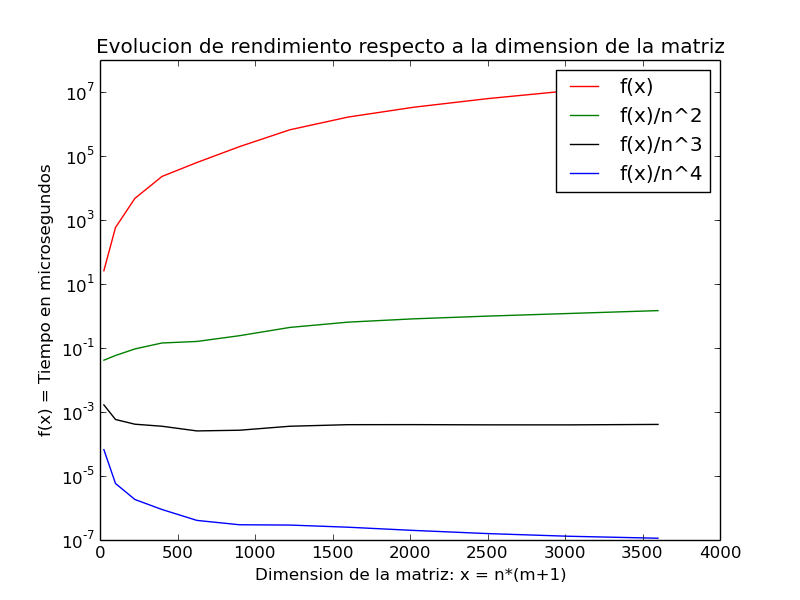
\includegraphics[scale=0.35]{experimentos2a_2b/tiempos_nm_fitteo_1_inst/factorizacion_lu_time_consumed.png}
\end{center}

A pesar de ser una heur\'istica, podemos corroborar que la curva sobre cubo se asemeja mucho a una constante, mientras que al cuadrado y a la cuarta funciones crecientes y decrecientes, respectivamente. Por lo que podemos decir que probamos emp\'iricamente que los algoritmos son del orden c\'ubico.

\subsubsection{Performance de EG vs LU variando la cantidad de instancias y la granularidad de la discretizacion}

Para comenzar esta seccion, compararemos la performance de EG vs LU variando las discretizaciones, con archivos de entrada de una sola instancia. A continuacion se presentan los graficos de comparación entre EG y LU, en diferentes escalas.

\begin{center}
\textbf{1 instancia por archivo de test}\\
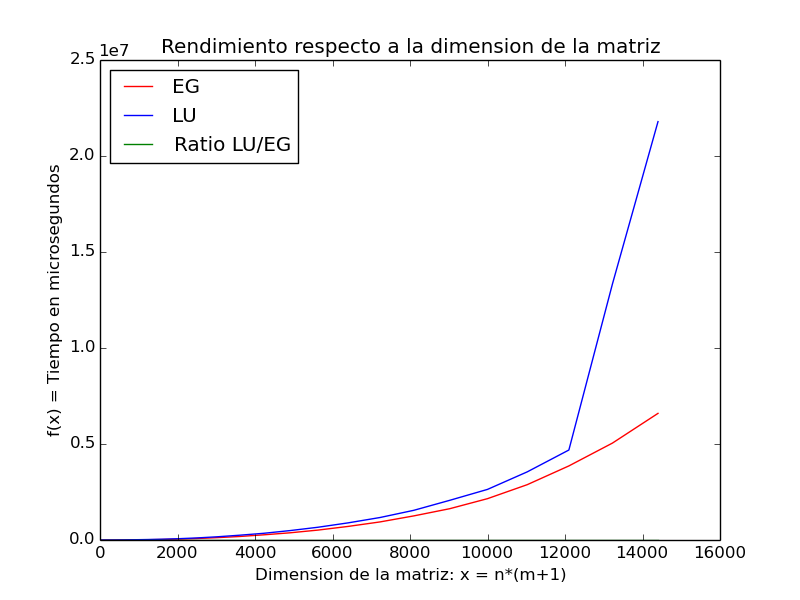
\includegraphics[scale=0.35]{experimentos2a_2b/tiempos_nm_fitteo_1_inst/gauss_vs_lu_time_consumed_abs.png}
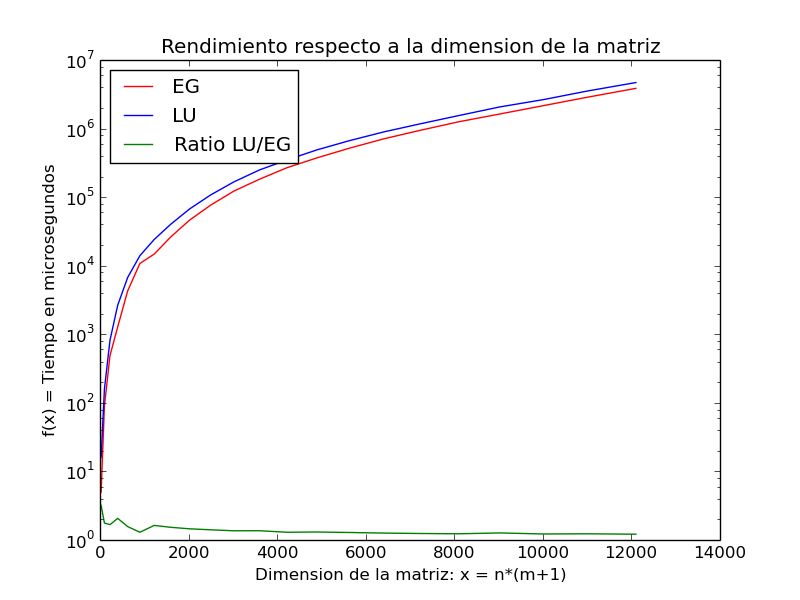
\includegraphics[scale=0.35]{experimentos2a_2b/tiempos_nm_fitteo_1_inst/gauss_vs_lu_time_consumed_log.png}
\end{center}

Dado que factorizacion LU, es identico a EG, pero guardando los coeficientes en la matriz L, tiene sentido que para una sola instancia sea mas costoso realizar la factorizacion lu y resolver el sistema que simplemente resolver usando EG.

\vspace{0.5cm}

A continuacion, se presentan graficos comparativos entre LU y EG para distintas cantidades de instancias. Lo que se observa es que, la brecha entre EG y LU se acentúa cada vez más a medida que aumenta la cantidad de instancias(ver gráficos con escala lineal). Esto se debe a que la complejidad teorica de resolver k instancias (misma matriz A, distinto vector b, en un sistema Ax=b) usando EG es $\mathcal{O}( k * (n + m)^3 )$. Por otro lado, la complejidad de resolver k instancias usando LU es $\mathcal{O}((n + m)^3 + k*(n + m)^2)$, es decir: Complejidad cúbica para hallar la descomposicion LU, y luego $k$ resoluciones de los sistemas triangulares $Ly=b$ y $Ux=y$ que cuestan orden cuadrático cada uno. 

\begin{center}
\textbf{10 instancias por archivo de test}\\
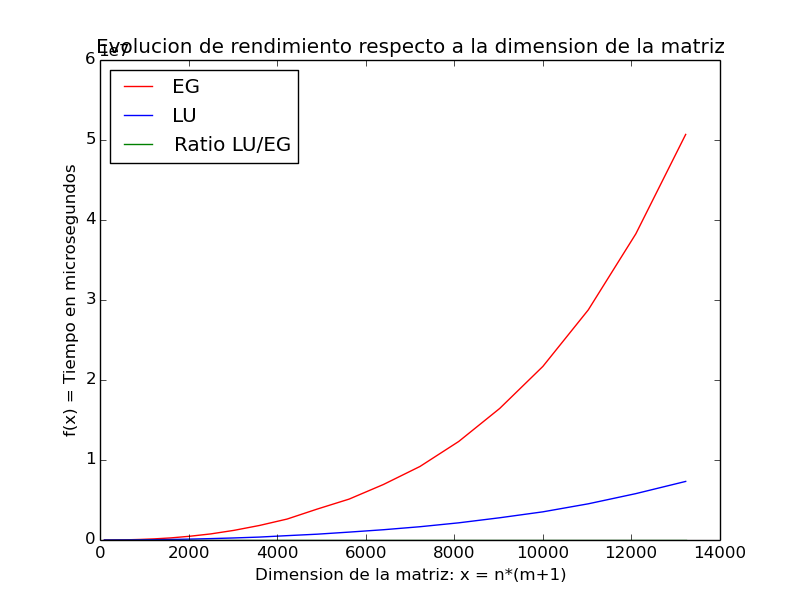
\includegraphics[scale=0.35]{experimentos2a_2b/gauss_vs_lu_10_inst/gauss_vs_lu_time_consumed_abs.png}
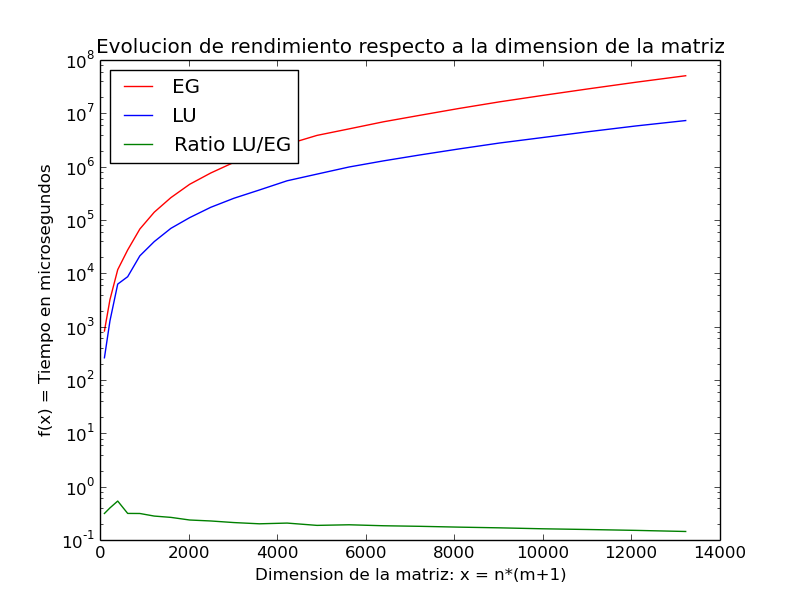
\includegraphics[scale=0.35]{experimentos2a_2b/gauss_vs_lu_10_inst/gauss_vs_lu_time_consumed_log.png}
\end{center}

\begin{center}
\textbf{50 instancias por archivo de test}\\
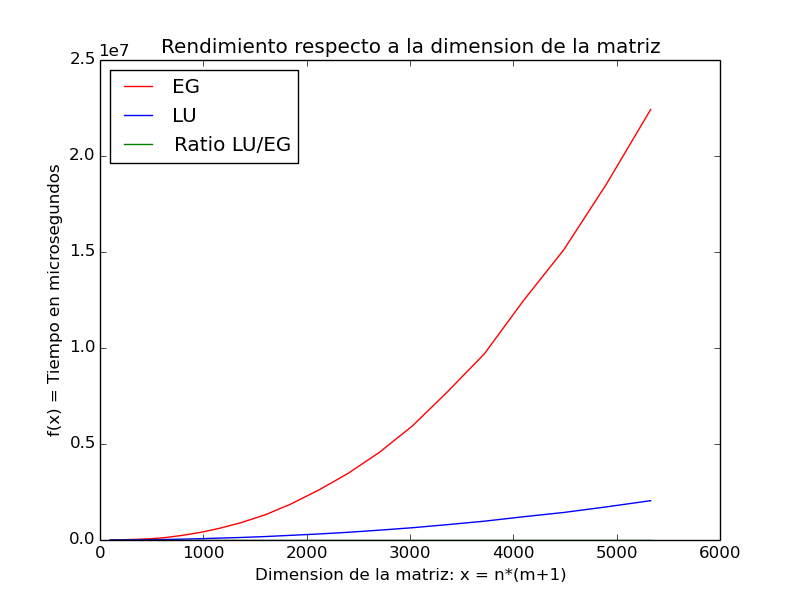
\includegraphics[scale=0.35]{experimentos2a_2b/gauss_vs_lu_50_inst/gauss_vs_lu_time_consumed_abs.png}
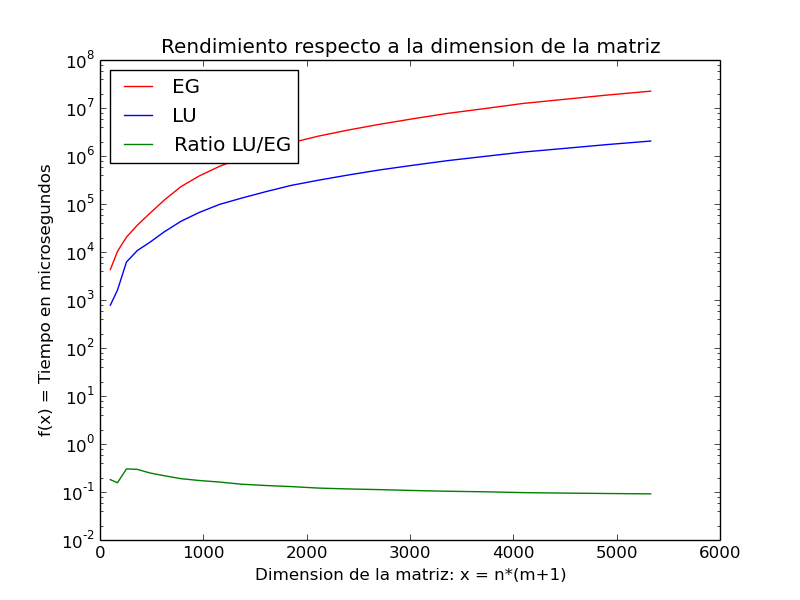
\includegraphics[scale=0.35]{experimentos2a_2b/gauss_vs_lu_50_inst/gauss_vs_lu_time_consumed_log.png}
\end{center}

\begin{center}
\textbf{150 instancias por archivo de test}\\
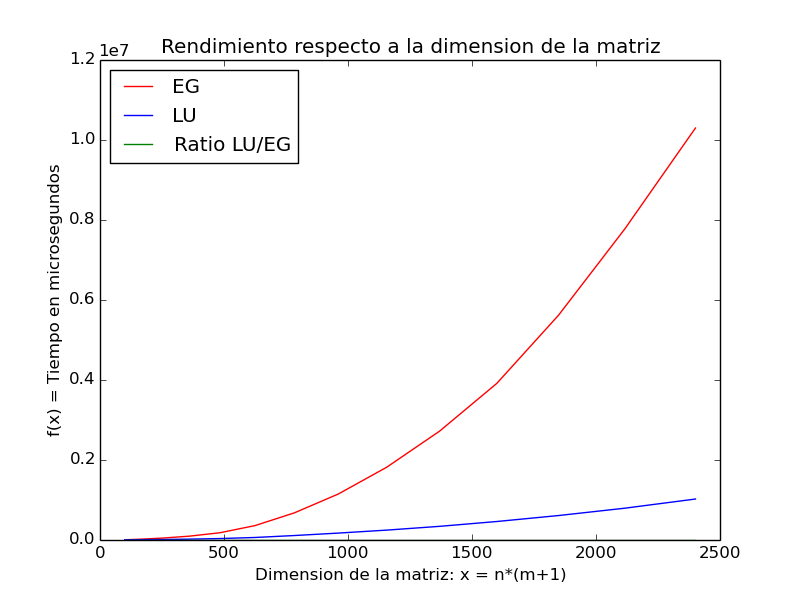
\includegraphics[scale=0.35]{experimentos2a_2b/gauss_vs_lu_150_inst/gauss_vs_lu_time_consumed_abs.png}
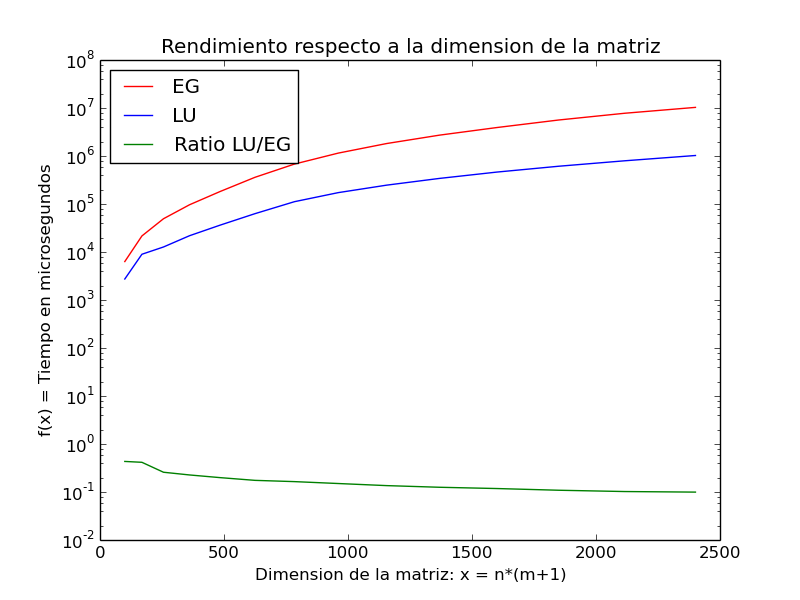
\includegraphics[scale=0.35]{experimentos2a_2b/gauss_vs_lu_150_inst/gauss_vs_lu_time_consumed_log.png}
\end{center}

\begin{center}
\textbf{500 instancias por archivo de test}\\
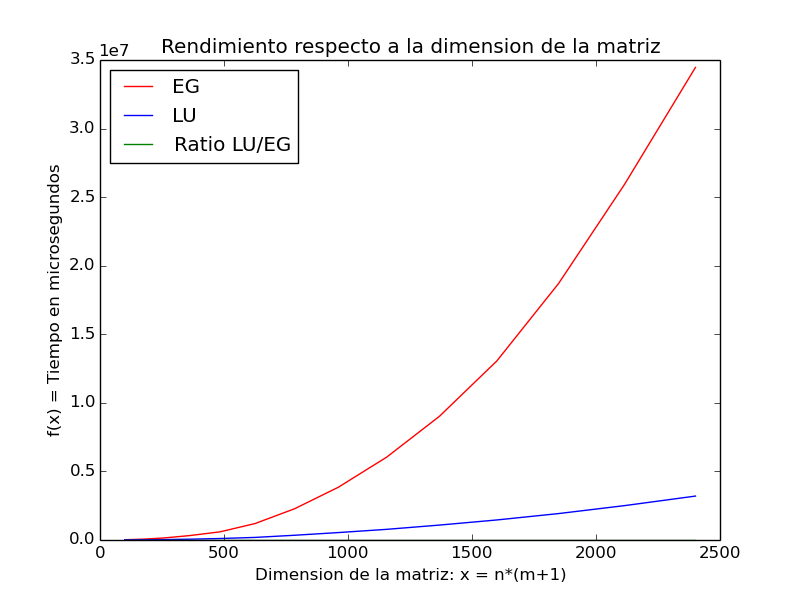
\includegraphics[scale=0.35]{experimentos2a_2b/gauss_vs_lu_500_inst/gauss_vs_lu_time_consumed_abs.png}
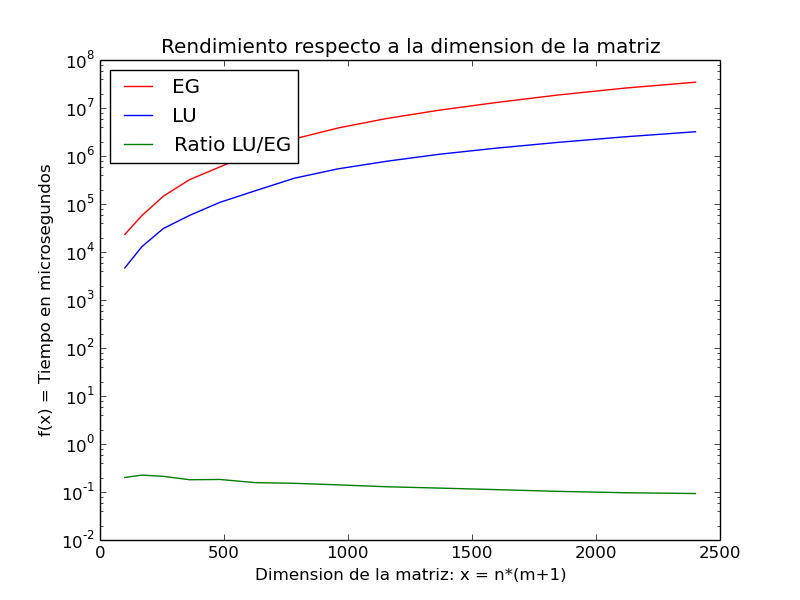
\includegraphics[scale=0.35]{experimentos2a_2b/gauss_vs_lu_500_inst/gauss_vs_lu_time_consumed_log.png}
\end{center}

Tambien se observa en los graficos con escala logaritmica que la brecha entre EG y LU para una cantidad de instancias fija se acentua a medida que se aumenta el tamaño de la matriz del sistema, pues el ratio LU/EG decrece. Creemos que esto se debe a que al dejar k fijo y aumentar $n+m$, tenemos que $\mathcal{O}((n + m)^3 + k*(n + m)^2)$ es mas pequeño que $\mathcal{O}(k*(n + m)^3)$ en terminos empíricos. 

\textbf{Consideraci\'on Adicional:} 

Luego de la experimentacion, se nos ocurrio una optimizacion de la implementaci\'on de los algoritmos, se agreg\'o la siguiente sentencia condicional al código de EG y la parte de triangulacion de LU:

\begin{lstlisting}
			.
			.
			.
for (int j = i+1; j < numfilas; j++) {

            if (abs(_A[j][i]) < EPSILON) {
                continue;
            }
			.
			.
			.
\end{lstlisting}

Es decir, si el elemento a analizar de la matriz es un cero(con tolerancia epsilon, en nuestro caso $exp(10, -9)$), el algoritmo no realiza el c\'alculo del coeficiente multiplicador ni tampoco opera sobre la fila multiplicando cada elemento por \'este. Al agregar esta sentencia y realizar los experimentos de fitteo de orden de complejidad, obtuvimos como resultado que la complejidad emp\'irica de ambos algoritmos era de orden cuadr\'atico. Creemos que esto se debe a la condición banda de la matriz, y que en muchos casos esta condición de corte evita que el algoritmo ingrese en la tercera iteracion anidada.

\subsubsection{Diferencia numérica de soluciones entre EG y LU}
En esta sección se mostraran los resultados de comparar las soluciones a un mismo sistema de ecuaciones $Ax=b$ usando LU y EG. Se realizo una variación en el tamaño de la matriz del sistema para ver la evolucion de las mediciones.\\

\vspace{0.3cm}

Los parámetros utilizados para el experimento fueron:
\begin{itemize}
	\item \textbf{Temperaturas internas y externas:}  externas(1500) e internas(100) \textbf{constantes} en todos los tests. 
	\item \textbf{Radio interno:} 200
	\item \textbf{Radio externo:} 400
	\item \textbf{Tamaño n de la matriz $A \in \mathbb{R}^{n \times n}$:} $[10^2\dots130^2]$
	\item \textbf{Isoterma buscada:} 500
\end{itemize}

No se mostrará ningun gráfico porque todas las mediciones de diferencia dieron cero, es decir:

\begin{itemize}
    \item $\norm{ x - \hat{x} }_\infty = 0.0 $
    \item $\norm{ x - \hat{x} }_2 = 0.0 $ 
\end{itemize}

Dado este sorprendente resultado a primera vista, hicimos un análisis mas fino del codigo y llegamos a algunas conclusiones:
\begin{itemize}
	\item El código de la resolución del problema es identico en ambos métodos desde la lectura de la entrada hasta el armado del sistema $Ax=b$, con lo cual no puede haber diferencia numérica en este tramo.
	\item El código de factorizacion lu y eliminacion gaussiana es \texttt{idéntico} salvo que LU guarda los multiplicadores en otra matriz L, tambien de precision doble, con lo cual lo único que podria acarrear LU contra EG en este tramo es el almacenamiento con error de los coeficientes.
	\item LU tambien podría acarrear error al realizar las 2 resoluciones de sistemas triangulares(contra una sola de EG)
\end{itemize}

Sin embargo, en los casos planteados esto no ocurre. Como futuro trabajo, se podrian fabricar casos de test muy especificos donde se fuercen errores numericos clásicos. (ie. sumas con números de distinto orden, restas con numeros muy cercanos, etc.) en las operaciones de resolucion de los sistemas triangulares, se esperaría que LU acarree mas error ya que realiza mas operaciones para resolver el sistema original $Ax=b$.

\subsubsection{Evolución estimación de la isoterma y temperatura}
Se presentarán los resultados de los experimentos en el mismo orden en que fueron planteados en la sección de desarrollo. Se realizará el análisis de los mismos en este mismo apartado.
\begin{enumerate}
	\item \begin{itemize}
				\item \textbf{Temperaturas internas y externas:} aleatorias uniformes entre $[50\dots200]$ y $[1450\dots1550]$, pero fijas entre tests.
				\item \textbf{Radio interno:} 200
				\item \textbf{Radio externo:} 400
				\item \textbf{Cantidad radios:} $[5\dots100]$
				\item \textbf{Cantidad ángulos:} 100
				\item \textbf{Isoterma buscada:} 500
			\end{itemize}
Se adjunta con el trabajo práctico un video que expone la evolución del sistema mientras se incrementa la cantidad de radios. Expondremos estáticamente algunos frames, pero es conveniente ver el video primero. Se encuentra en la misma carpeta que el pdf. (variación\_radial\_isomap.mp4, variación\_radial\_heatmap.mp4).

\vspace{0.5cm}

  	\textbf{Variación de la estimación de la isoterma entre 5 y 6 radios de discretización}\\
	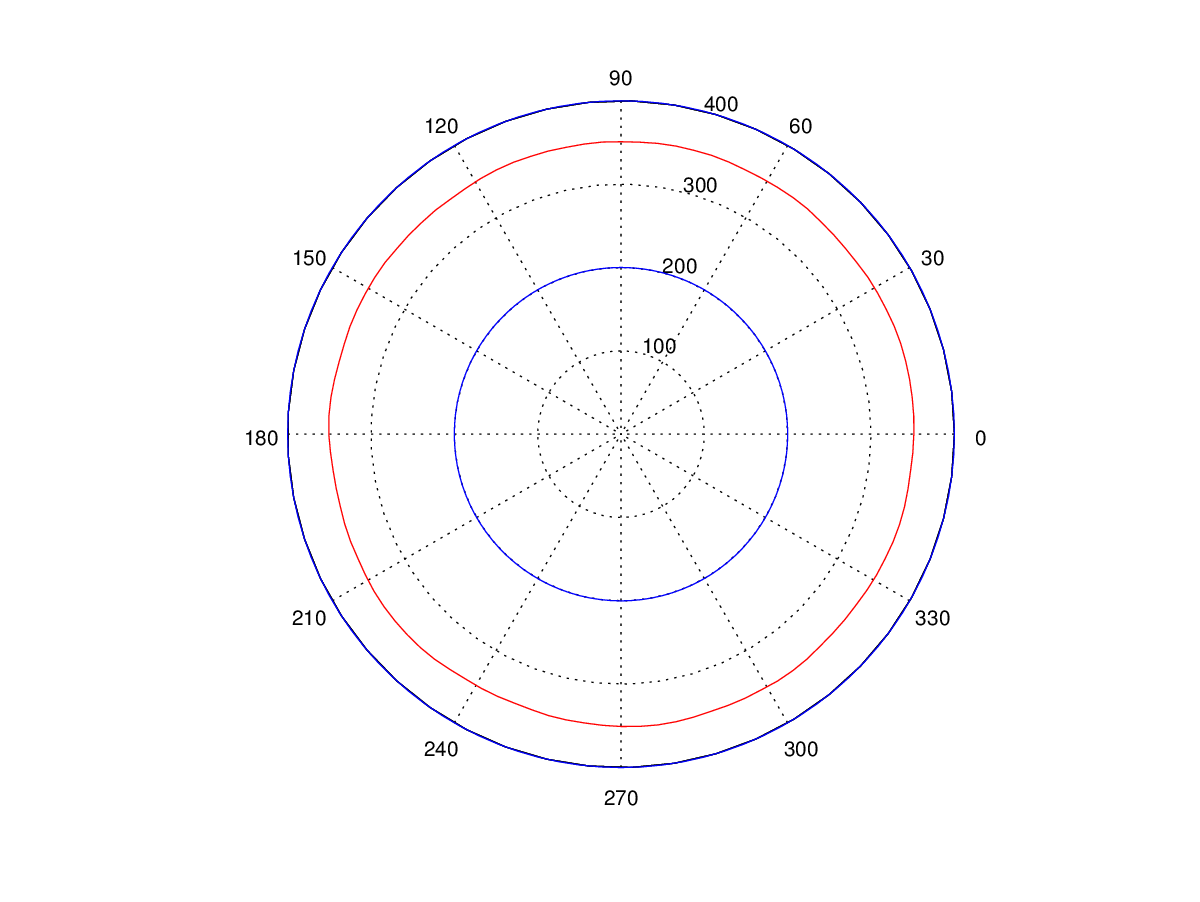
\includegraphics[scale=0.35]{experimentos1a_1b/evolucion_posicion_isoterma_temperatura/test2/test6_006_radios_inst_001_isomap.png}
	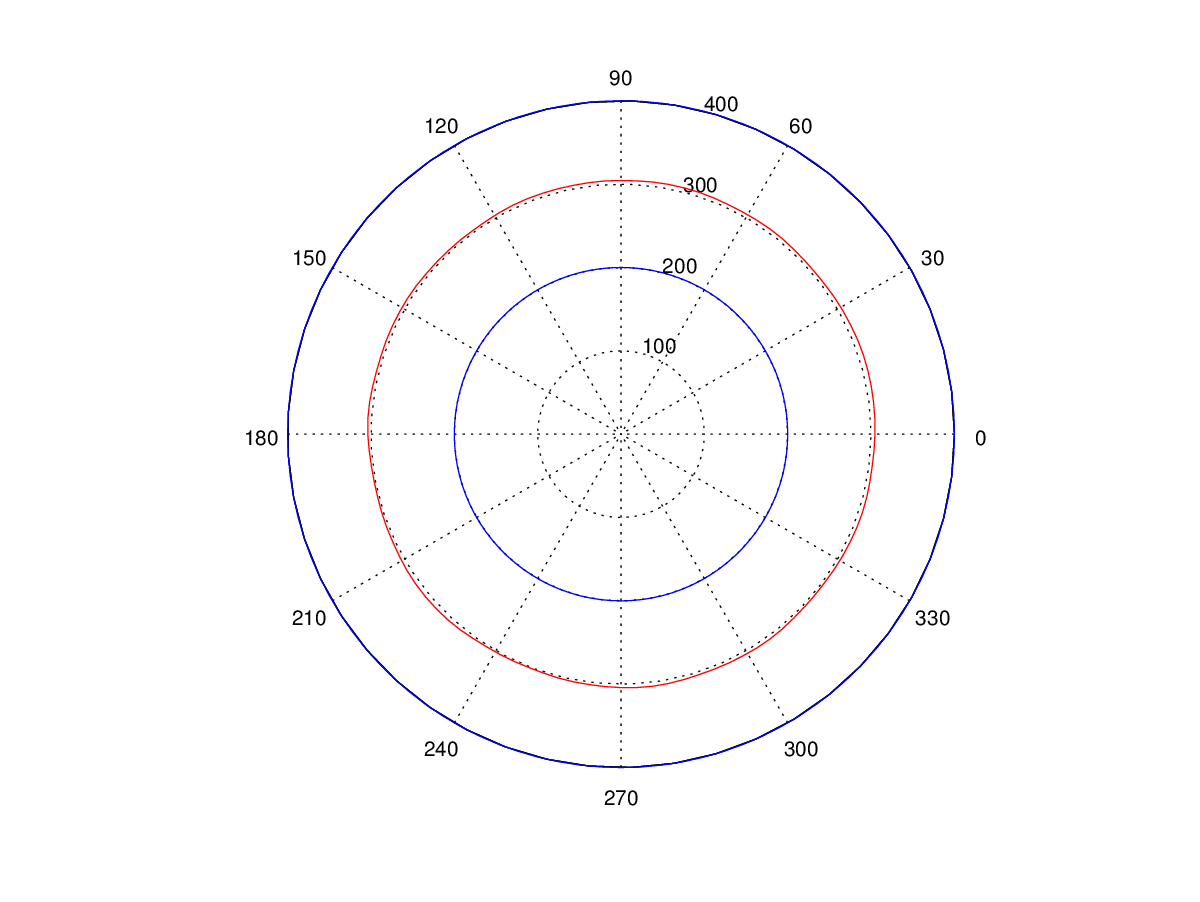
\includegraphics[scale=0.35]{experimentos1a_1b/evolucion_posicion_isoterma_temperatura/test2/test6_007_radios_inst_001_isomap.png}
	
  	\textbf{Variación de la temperatura entre 6 y 7 radios de discretización}\\
	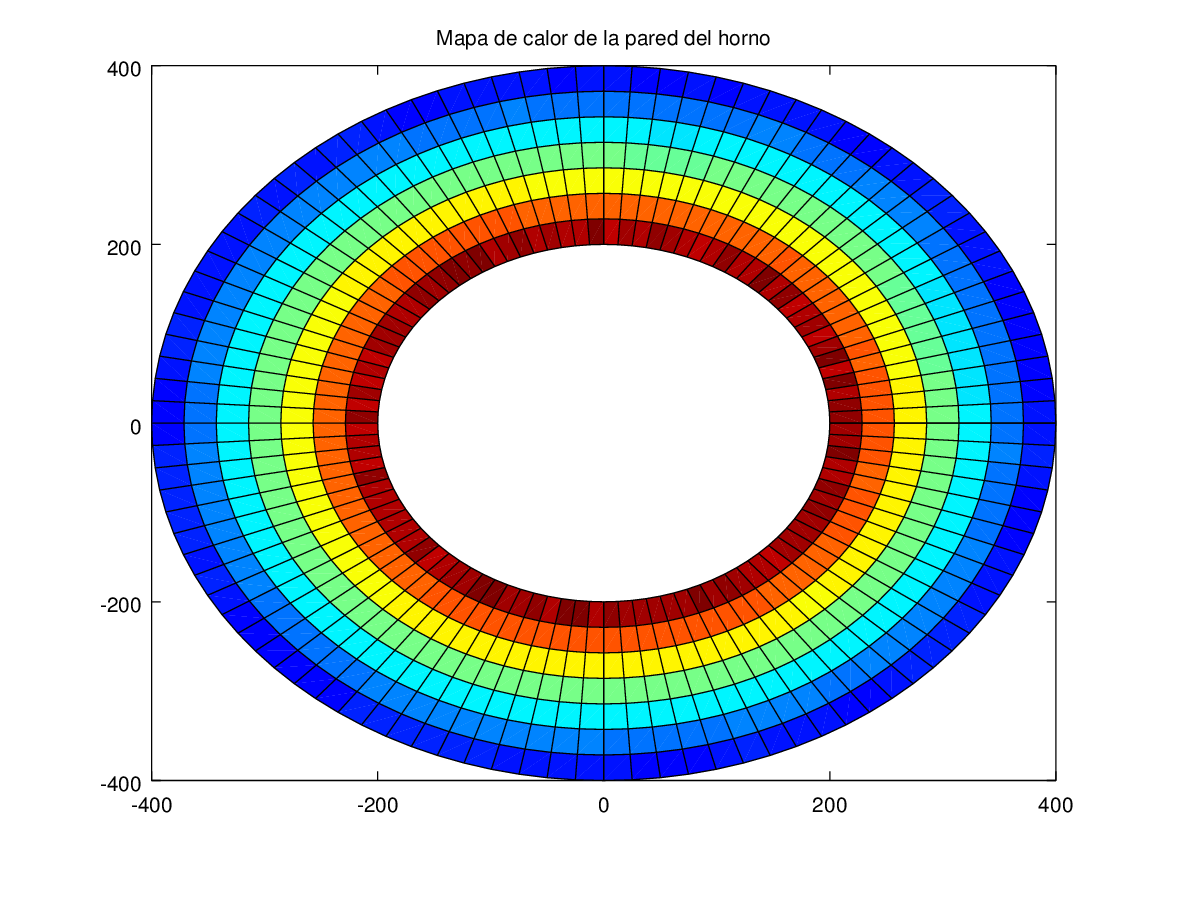
\includegraphics[scale=0.35]{experimentos1a_1b/evolucion_posicion_isoterma_temperatura/test2/test6_006_radios_inst_001_heatmap.png}
	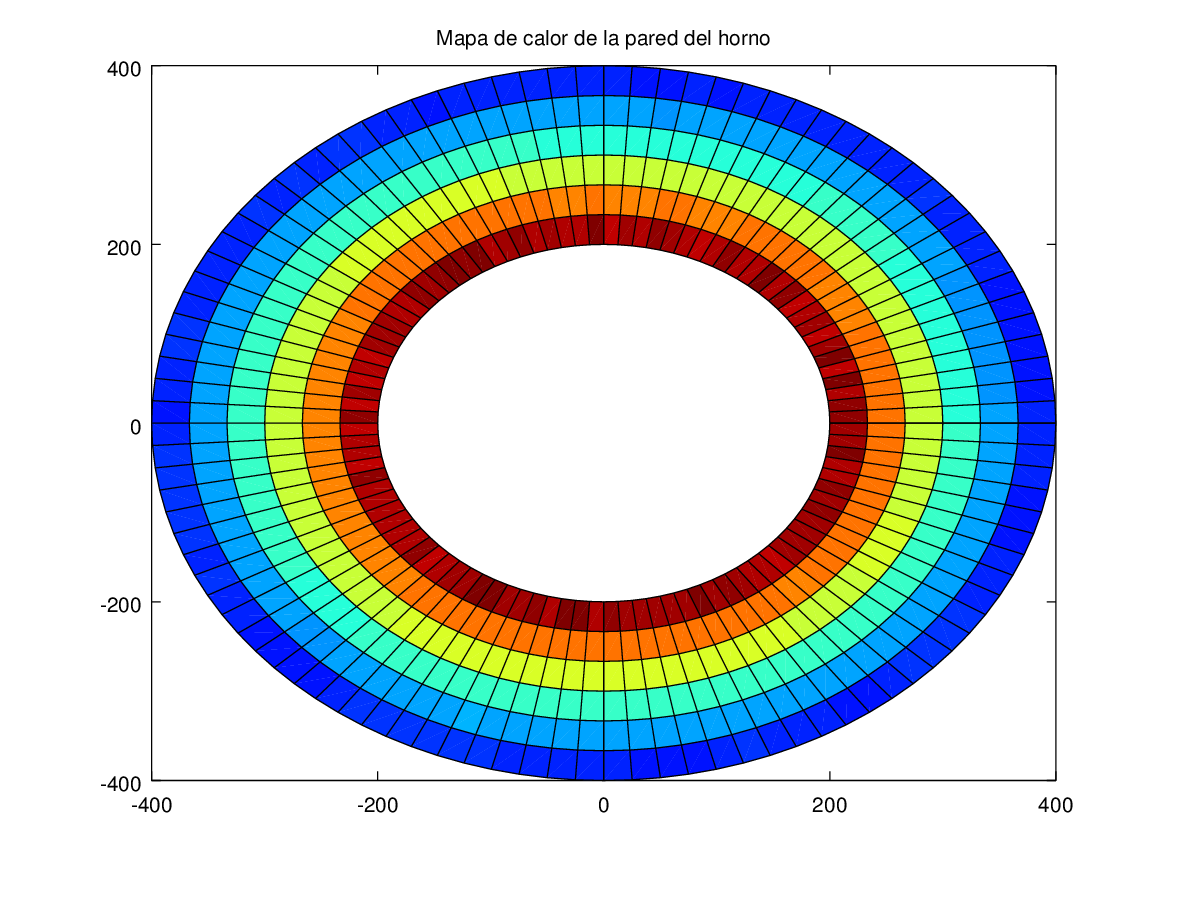
\includegraphics[scale=0.35]{experimentos1a_1b/evolucion_posicion_isoterma_temperatura/test2/test6_007_radios_inst_001_heatmap.png}

 	\textbf{Variación de la estimación de la isoterma entre 99 y 100 radios de discretización}\\
	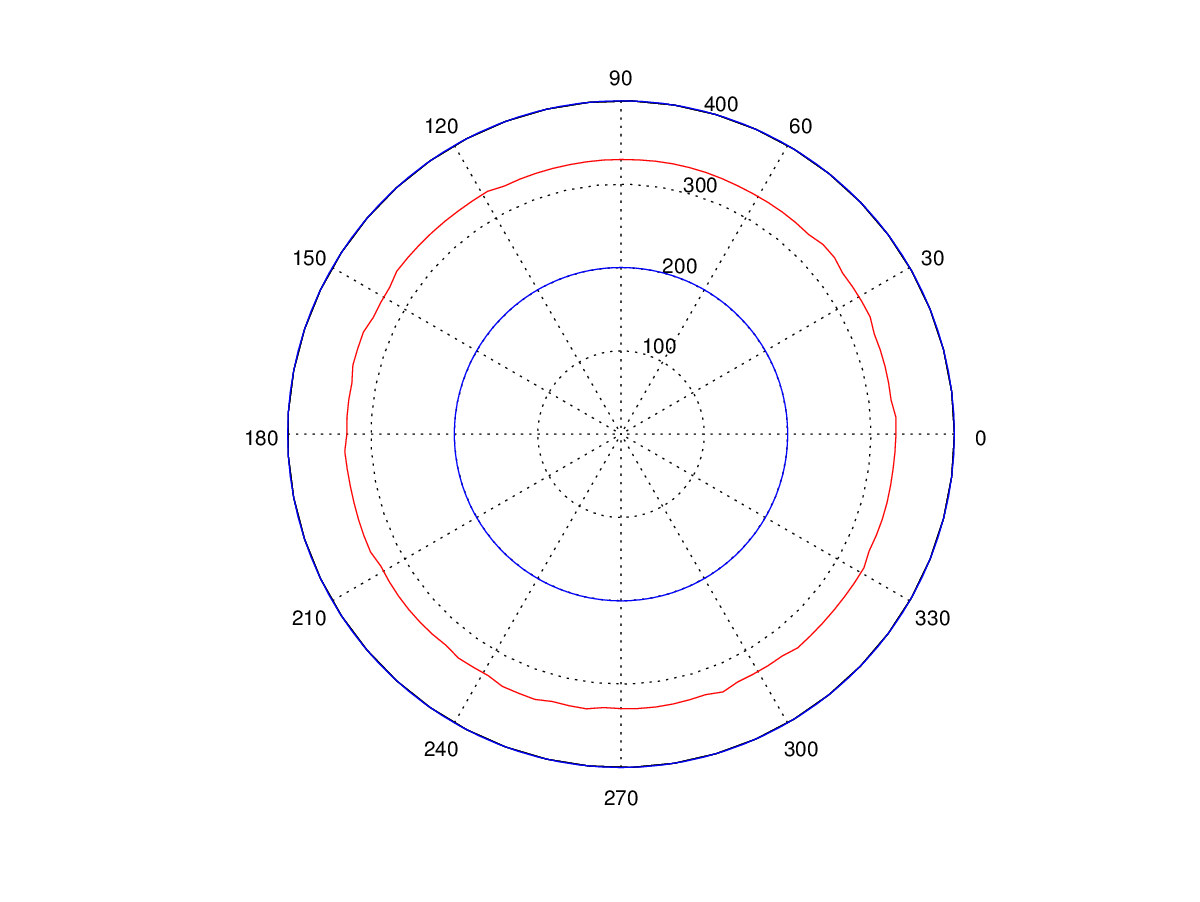
\includegraphics[scale=0.35]{experimentos1a_1b/evolucion_posicion_isoterma_temperatura/test2/test6_099_radios_inst_001_isomap.png}
	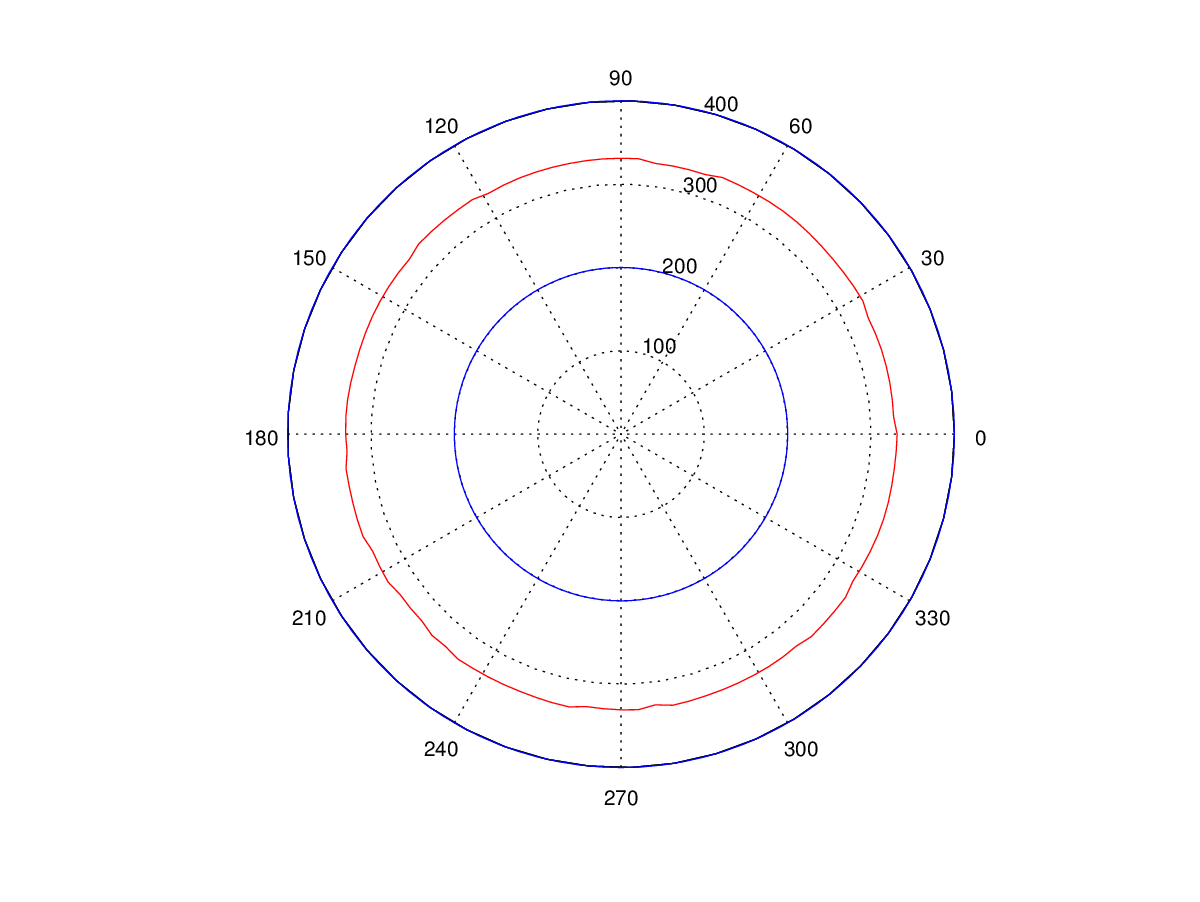
\includegraphics[scale=0.35]{experimentos1a_1b/evolucion_posicion_isoterma_temperatura/test2/test6_100_radios_inst_001_isomap.png}
	
	\textbf{Variación de la temperatura entre 99 y 100 radios de discretización}\\
	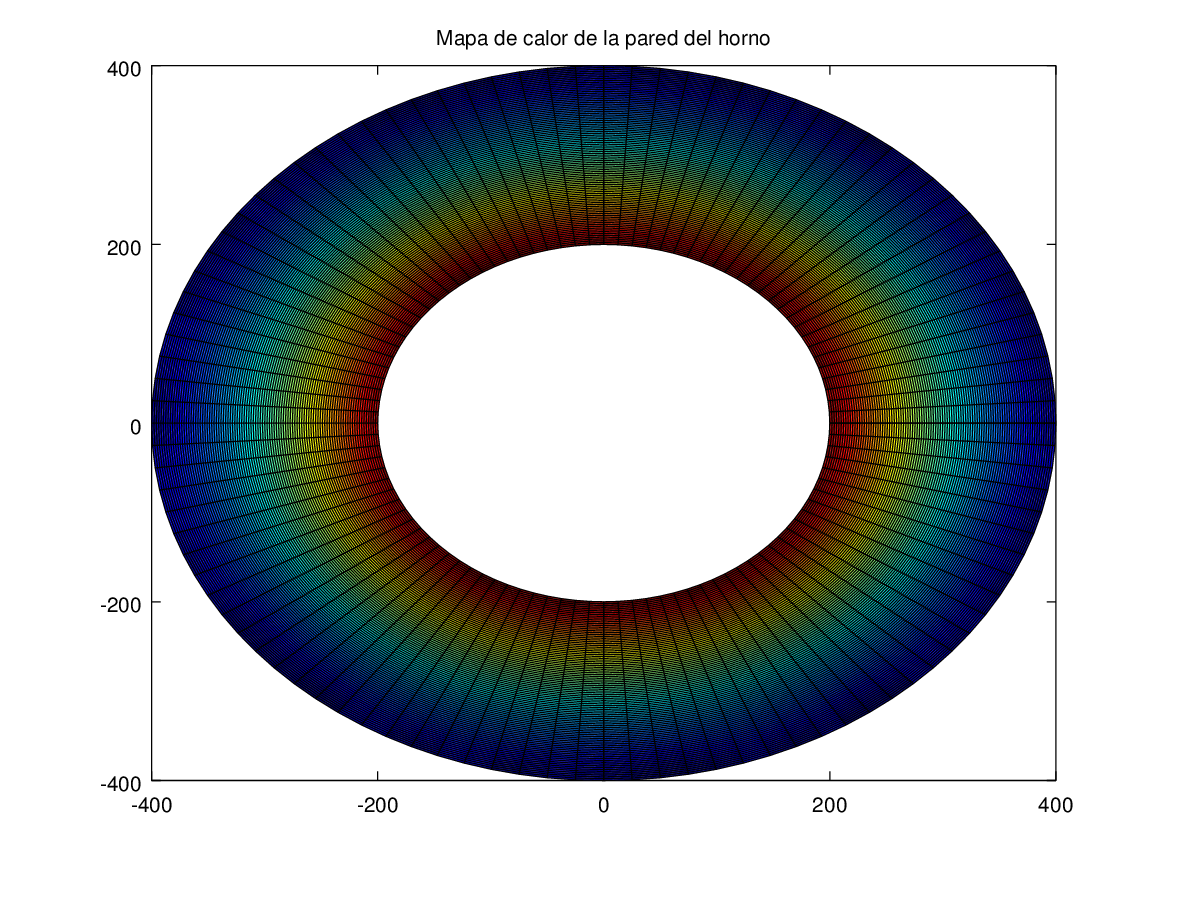
\includegraphics[scale=0.35]{experimentos1a_1b/evolucion_posicion_isoterma_temperatura/test2/test6_099_radios_inst_001_heatmap.png}
	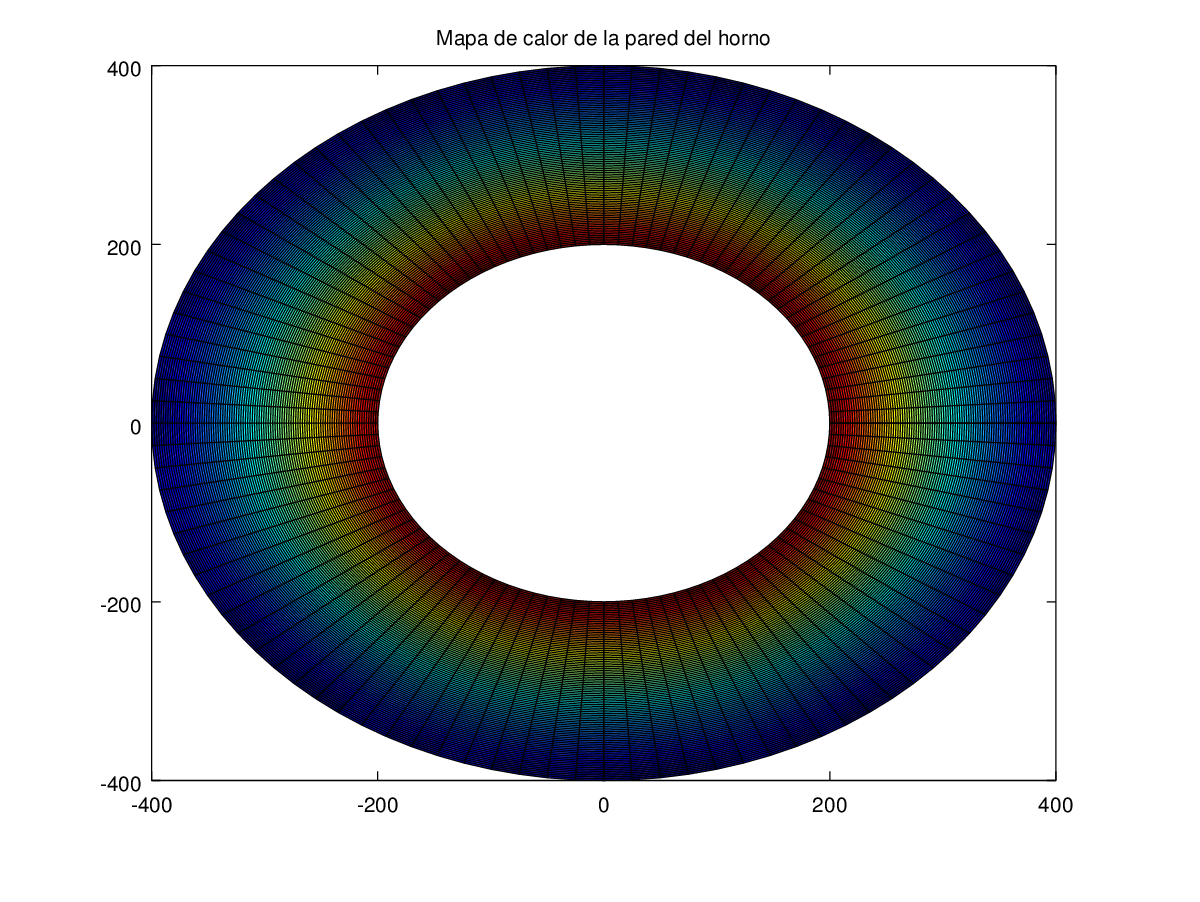
\includegraphics[scale=0.35]{experimentos1a_1b/evolucion_posicion_isoterma_temperatura/test2/test6_100_radios_inst_001_heatmap.png}

\vspace{0.5cm}

Se observa es que a medida que se aumenta la cantidad de radios de la discretización, la variación radial de la curva de la isoterma disminuye entre tests, es decir, se hace más fina la estimación, de forma tal que entre $i$ e $i+1$ radios la diferencia de la posición de la isoterma es menor a medida que $i$ crece. Para ver mejor esto se graficaron, para cada test de $i$ cantidad de radios de la discretización, el máximo y el promedio radial de la isoterma.

	\textbf{Evolución de la variación radial de la isoterma con cantidad creciente de radios}\\
	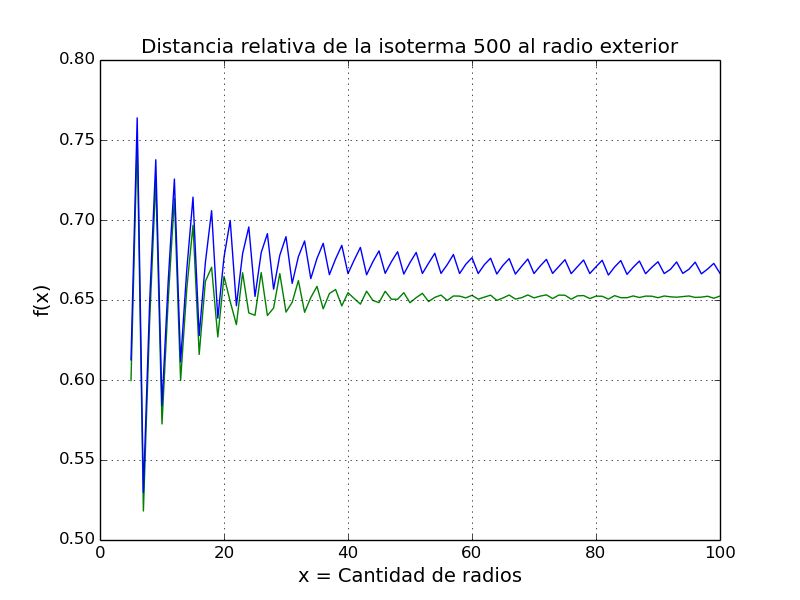
\includegraphics[scale=0.5]{experimentos1a_1b/evolucion_estimacion_seguridad_isoterma/100ang_5to100radios.png}\\


Para evitar distorsiones en el experimento anterior, se realizo otro muy similar al anterior pero con condiciones de borde \textbf{constantes e iguales}.
\begin{itemize}
	\item \textbf{Temperaturas internas y externas:} constantes, 100 y 1500. Esto es para que tenga la misma solución cada test del experimento.
	\item \textbf{Radio interno:} 200
	\item \textbf{Radio externo:} 400
	\item \textbf{Cantidad radios:} $[10\dots200]$
	\item \textbf{Cantidad ángulos:} 75
	\item \textbf{Isoterma buscada:} 500
\end{itemize}

No expondremos los resultados acerca de la evolucion de la temperatura y posicion de la isoterma, pues son similares al experimento anterior, la isoterma converge a medida que aumenta la cantidad de radios utilizada en la discretización. Al ser temperaturas constantes en este caso, la isoterma es un círculo perfecto. En el experimento anterior, la isoterma tenia pequeñas(casi imperceptibles) irregularidades dadas las condiciones aleatorias(con baja varianza) de borde.

\vspace{0.3cm}

Respecto al gráfico del promedio/maximo de la isoterma a medida que aumentan los radios, se tiene lo siguiente.

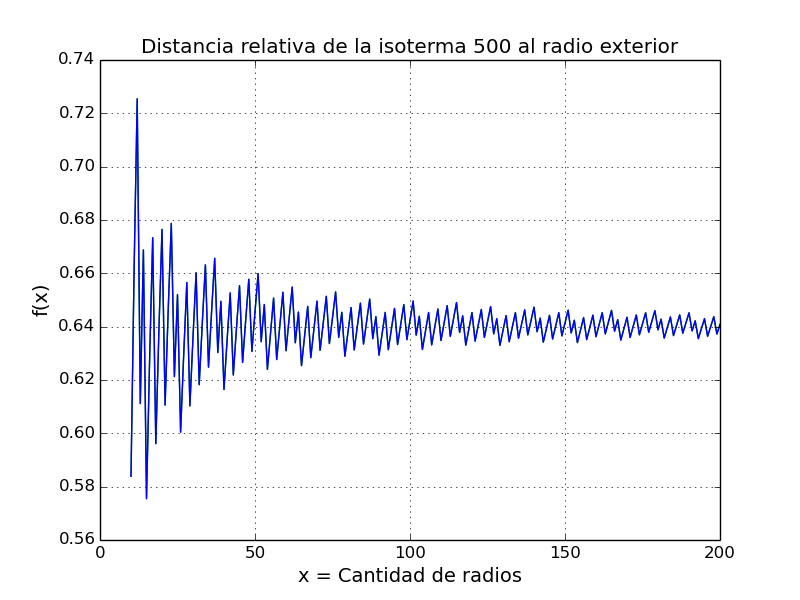
\includegraphics[scale=0.5]{experimentos1a_1b/evolucion_estimacion_seguridad_isoterma/75ang_10to200rad_evol_maxpromradio.png}\\
\textbf{Nota:} Al ser las condiciones de borde iguales, la isoterma tiene radio constante para cada experimento, con lo cual maximo y promedio coinciden, con lo cual se ve una sola curva.

\vspace{0.2cm}

Se puede ver que, al igual que en el experimento anterior, al aumentar la cantidad de radios, la posicion de la isoterma converge. Tambien se observa que en ambos experimentos, la posicion relativa de la isoterma converge aproximadamente a 0.64/0.66, lo cual tiene sentido ya que el experimento anterior tenia temperaturas aleatorias uniformes, pero \texttt{casi} alrededor de las temperaturas fijadas en el segundo experimento.\\

	\item \begin{itemize}
					\item \textbf{Temperaturas internas y externas:} constantes, 100 y 1500. Esto es para que tenga la misma solución cada test del experimento.
					\item \textbf{Radio interno:} 200
					\item \textbf{Radio externo:} 400
					\item \textbf{Cantidad radios:} 50
					\item \textbf{Cantidad ángulos:} $[5\dots50]$
					\item \textbf{Isoterma buscada:} 500
				\end{itemize}
	Se adjunta con el trabajo práctico un video que expone la evolución del sistema mientras se incrementa la cantidad de radios. Expondremos estáticamente algunos frames, pero es conveniente ver el video primero. Se encuentra en la misma carpeta que el pdf. (variación\_angular\_isomap.mp4, variación\_angular\_heatmap.mp4).

	\vspace{0.5cm}
	  	\textbf{Variación de la estimación de la isoterma entre 5 y 6 ángulos de discretización}\\
		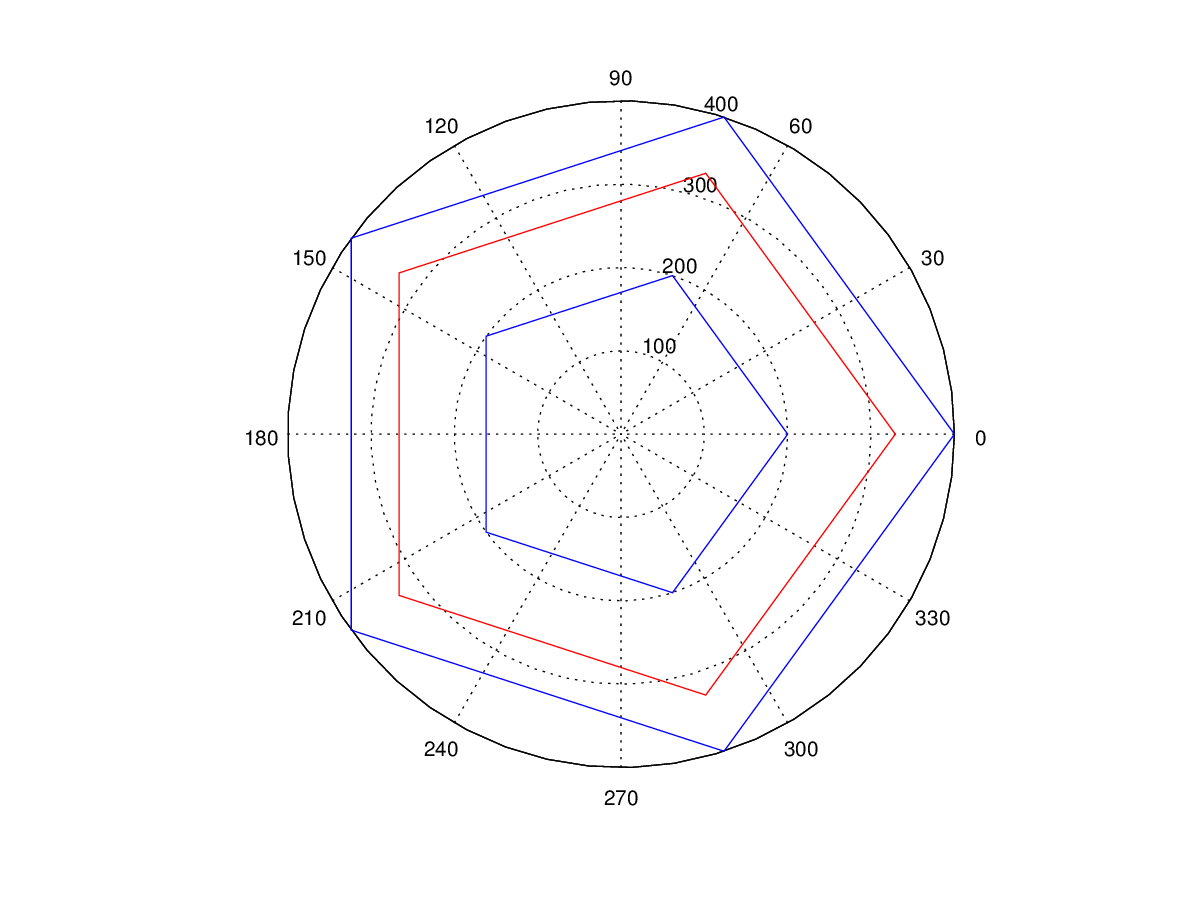
\includegraphics[scale=0.35]{experimentos1a_1b/evolucion_posicion_isoterma_temperatura/variacion_angulos_radio_fijo_se_suaviza_isoterma/test10_050_radios_005_angulos_inst_001_isomap.png}
		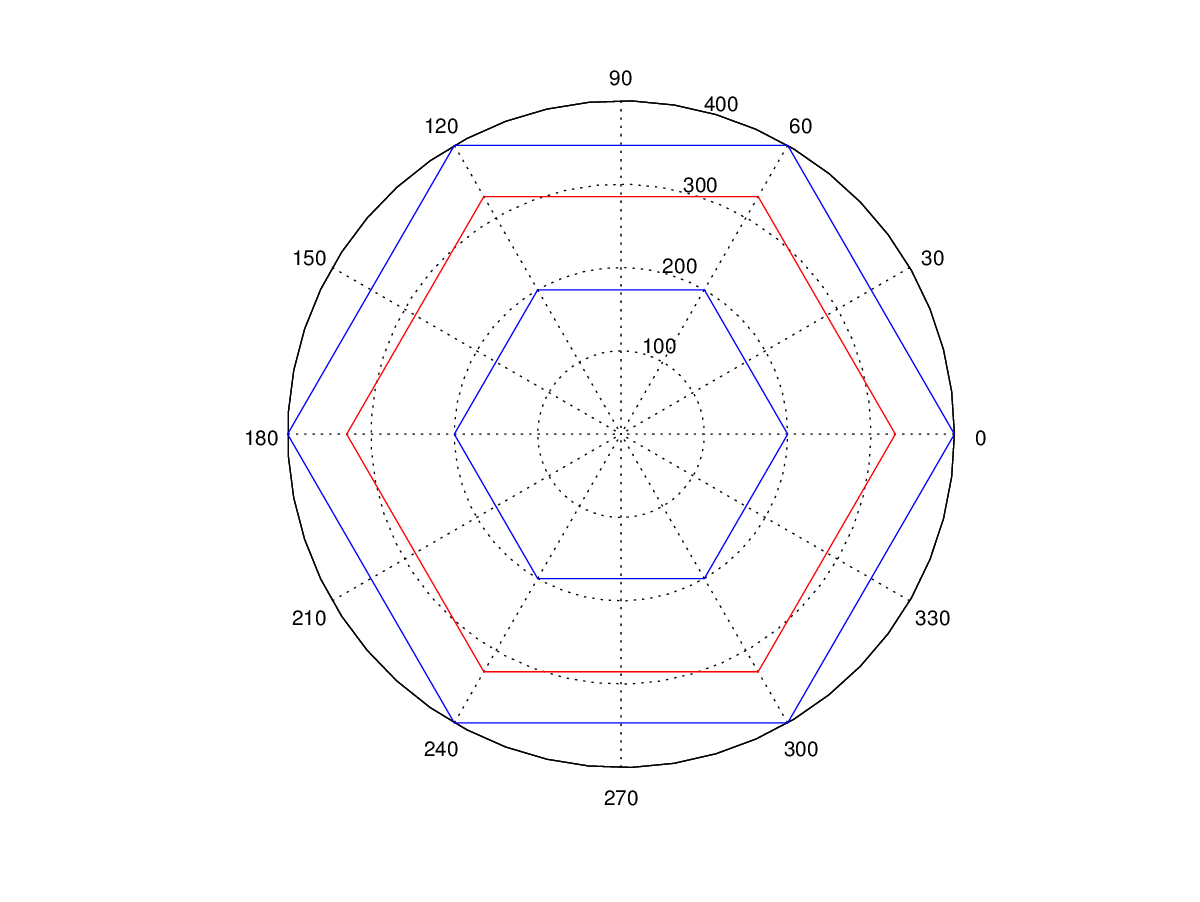
\includegraphics[scale=0.35]{experimentos1a_1b/evolucion_posicion_isoterma_temperatura/variacion_angulos_radio_fijo_se_suaviza_isoterma/test10_050_radios_006_angulos_inst_001_isomap.png}

	  	\textbf{Variación de la temperatura entre 5 y 6 ángulos de discretización}\\
	  	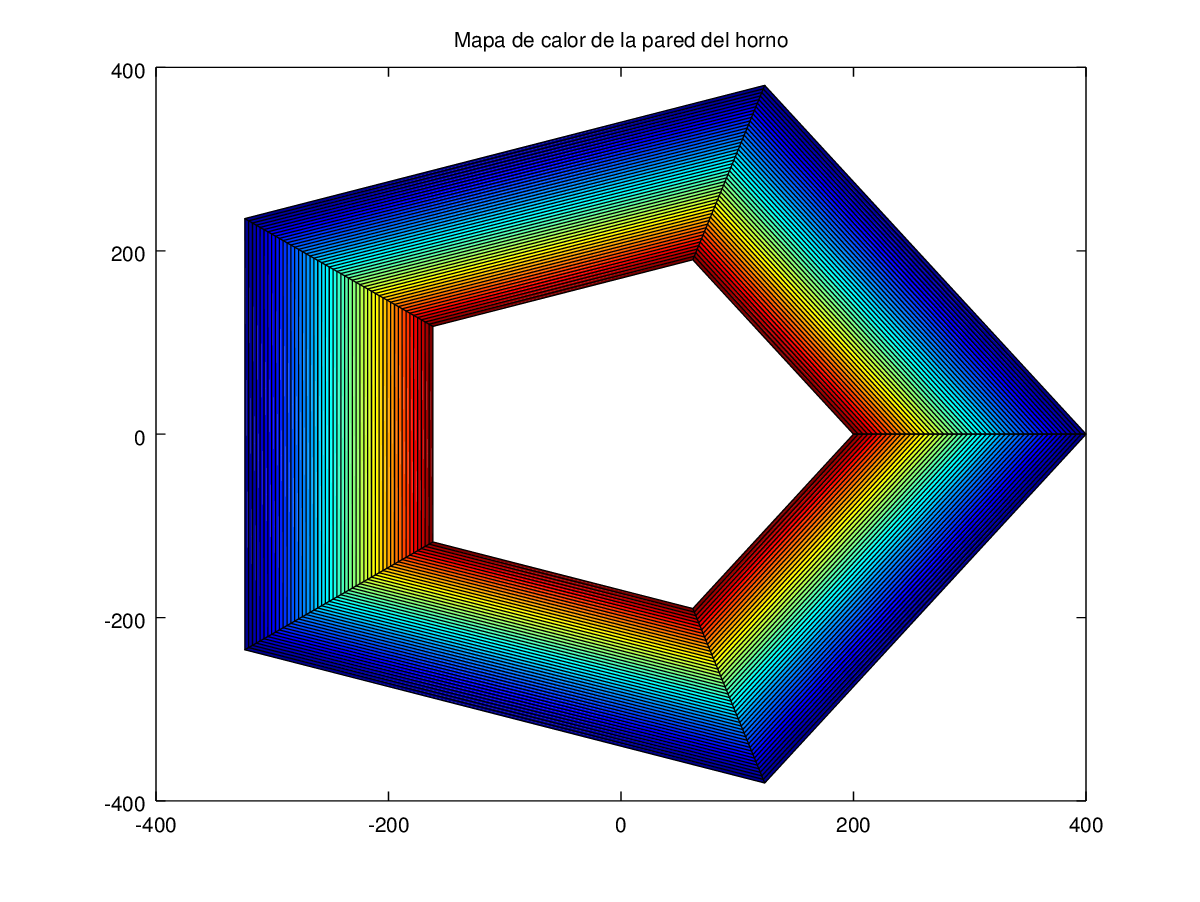
\includegraphics[scale=0.35]{experimentos1a_1b/evolucion_posicion_isoterma_temperatura/variacion_angulos_radio_fijo_se_suaviza_isoterma/test10_050_radios_005_angulos_inst_001_heatmap.png}
		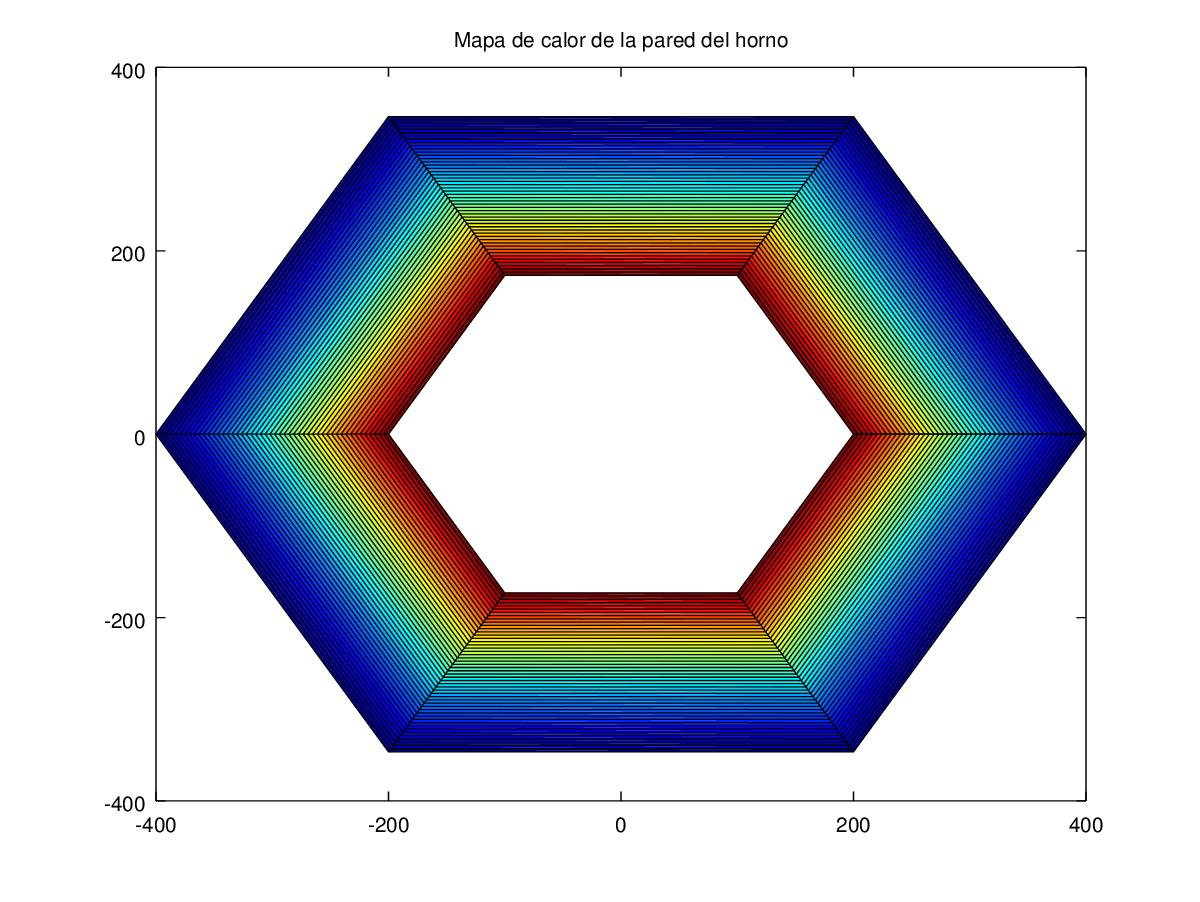
\includegraphics[scale=0.35]{experimentos1a_1b/evolucion_posicion_isoterma_temperatura/variacion_angulos_radio_fijo_se_suaviza_isoterma/test10_050_radios_006_angulos_inst_001_heatmap.png}	  	

	  	\textbf{Variación de la estimación de la isoterma entre 49 y 50 ángulos de discretización}\\
		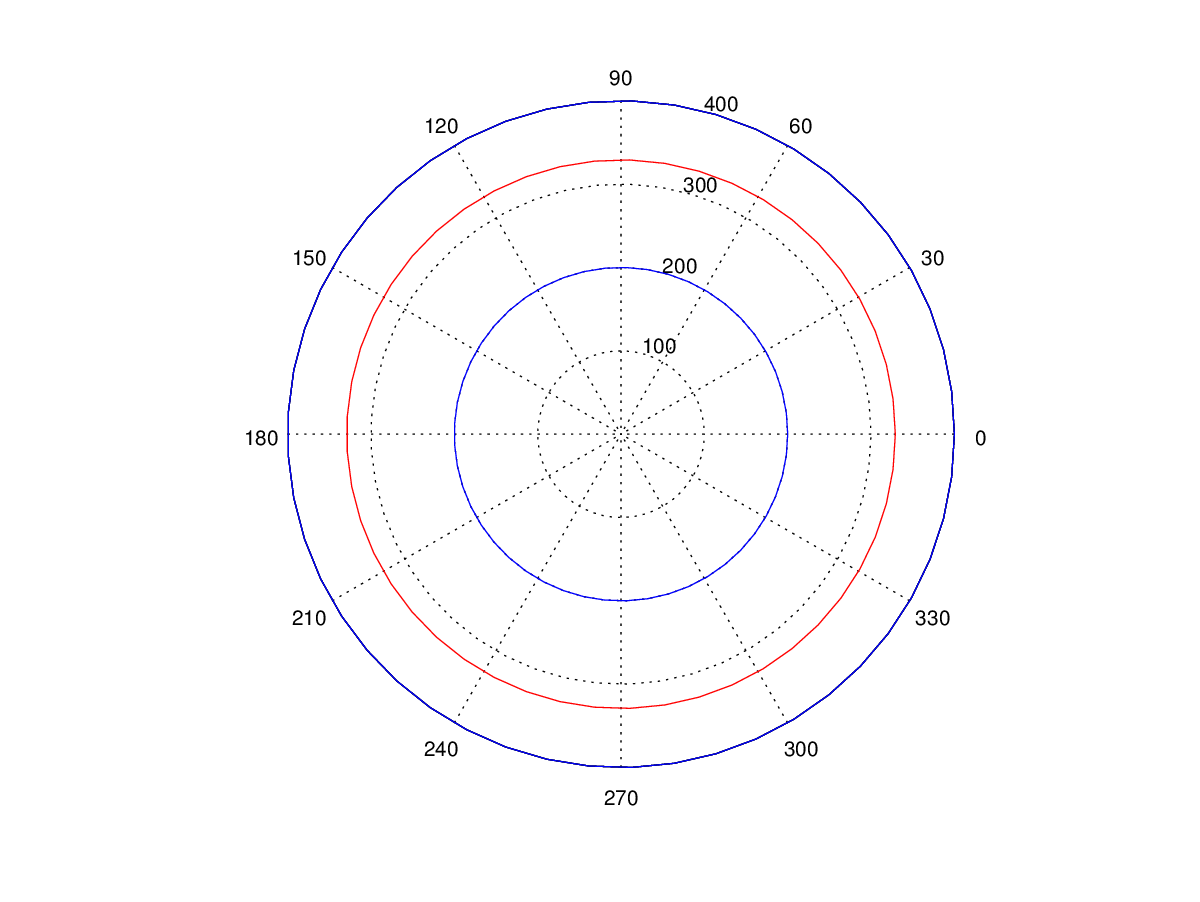
\includegraphics[scale=0.35]{experimentos1a_1b/evolucion_posicion_isoterma_temperatura/variacion_angulos_radio_fijo_se_suaviza_isoterma/test10_050_radios_049_angulos_inst_001_isomap.png}
		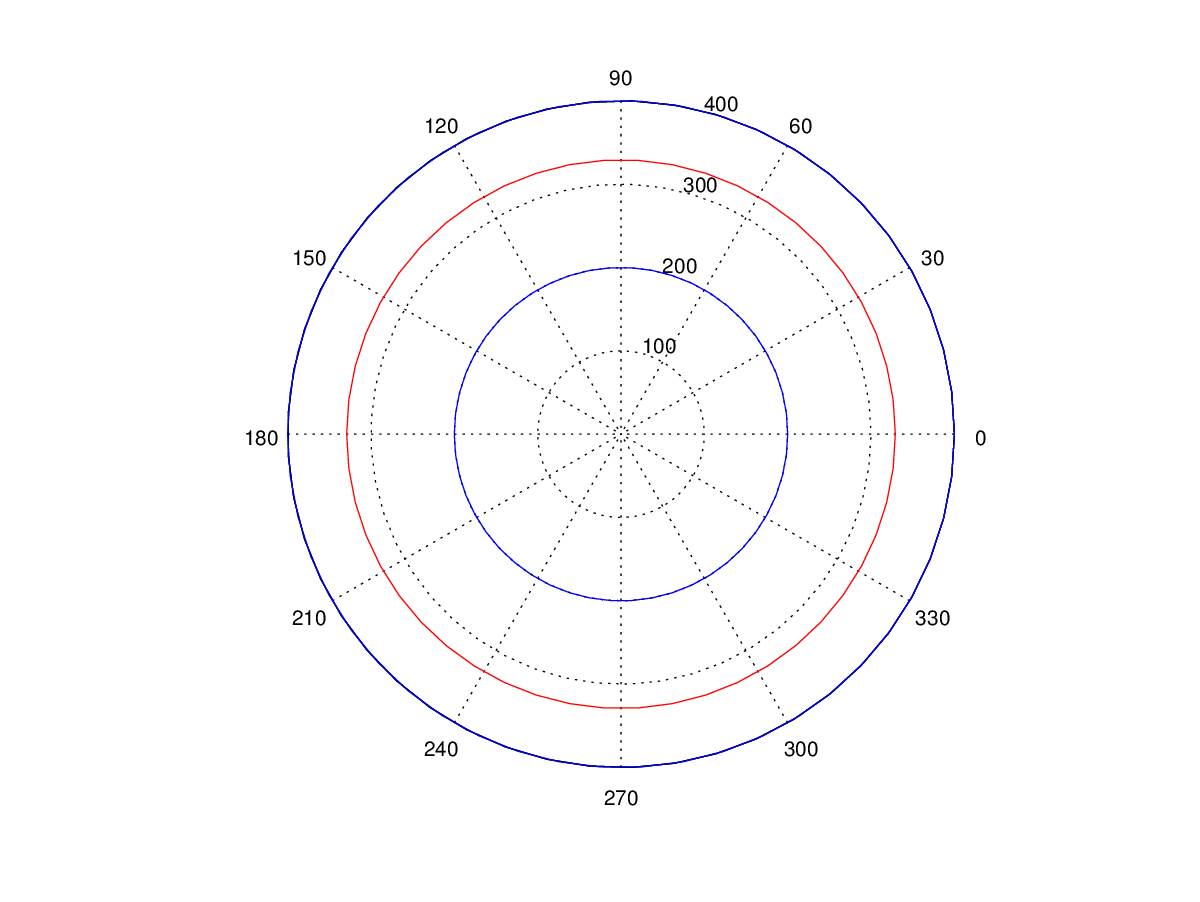
\includegraphics[scale=0.35]{experimentos1a_1b/evolucion_posicion_isoterma_temperatura/variacion_angulos_radio_fijo_se_suaviza_isoterma/test10_050_radios_050_angulos_inst_001_isomap.png}

		\textbf{Variación de la temperatura entre 49 y 50 ángulos de discretización}\\
	  	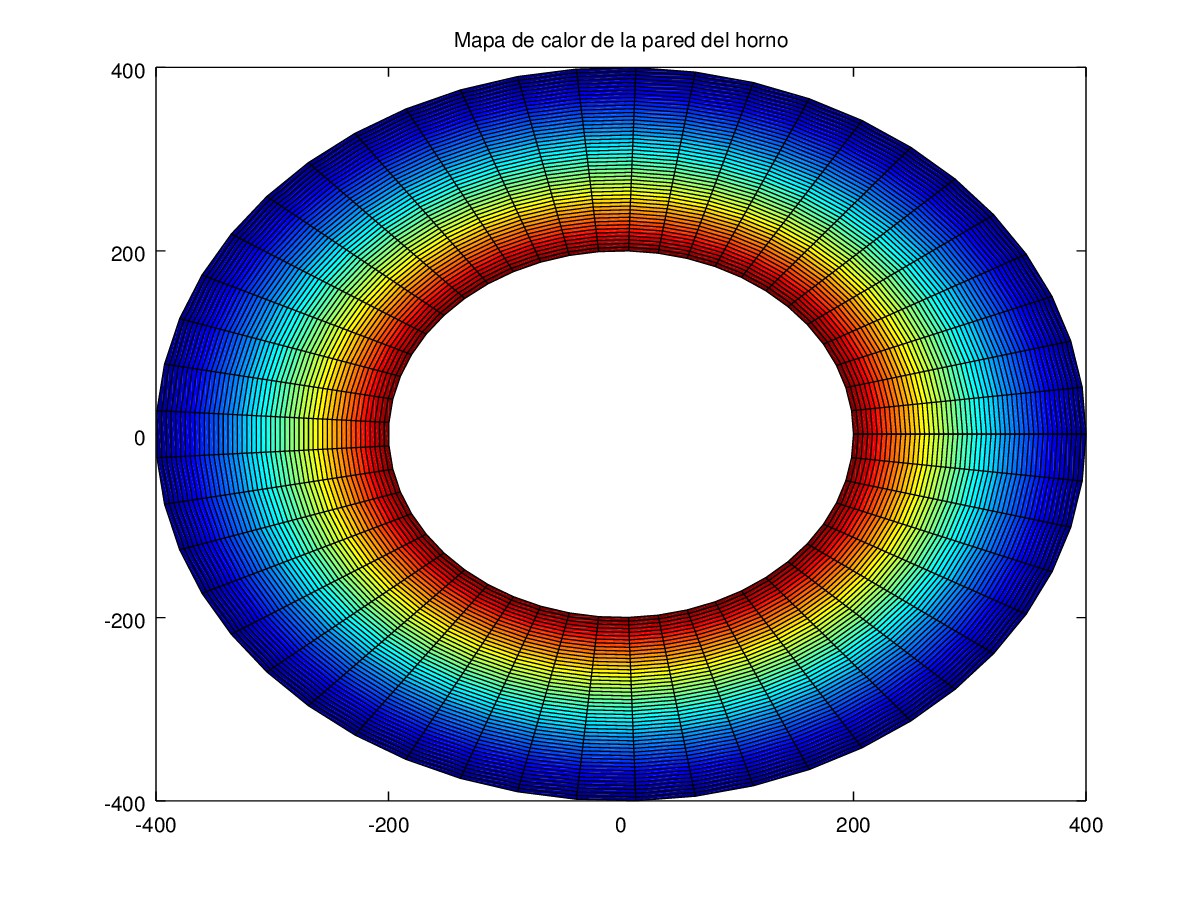
\includegraphics[scale=0.35]{experimentos1a_1b/evolucion_posicion_isoterma_temperatura/variacion_angulos_radio_fijo_se_suaviza_isoterma/test10_050_radios_049_angulos_inst_001_heatmap.png}
		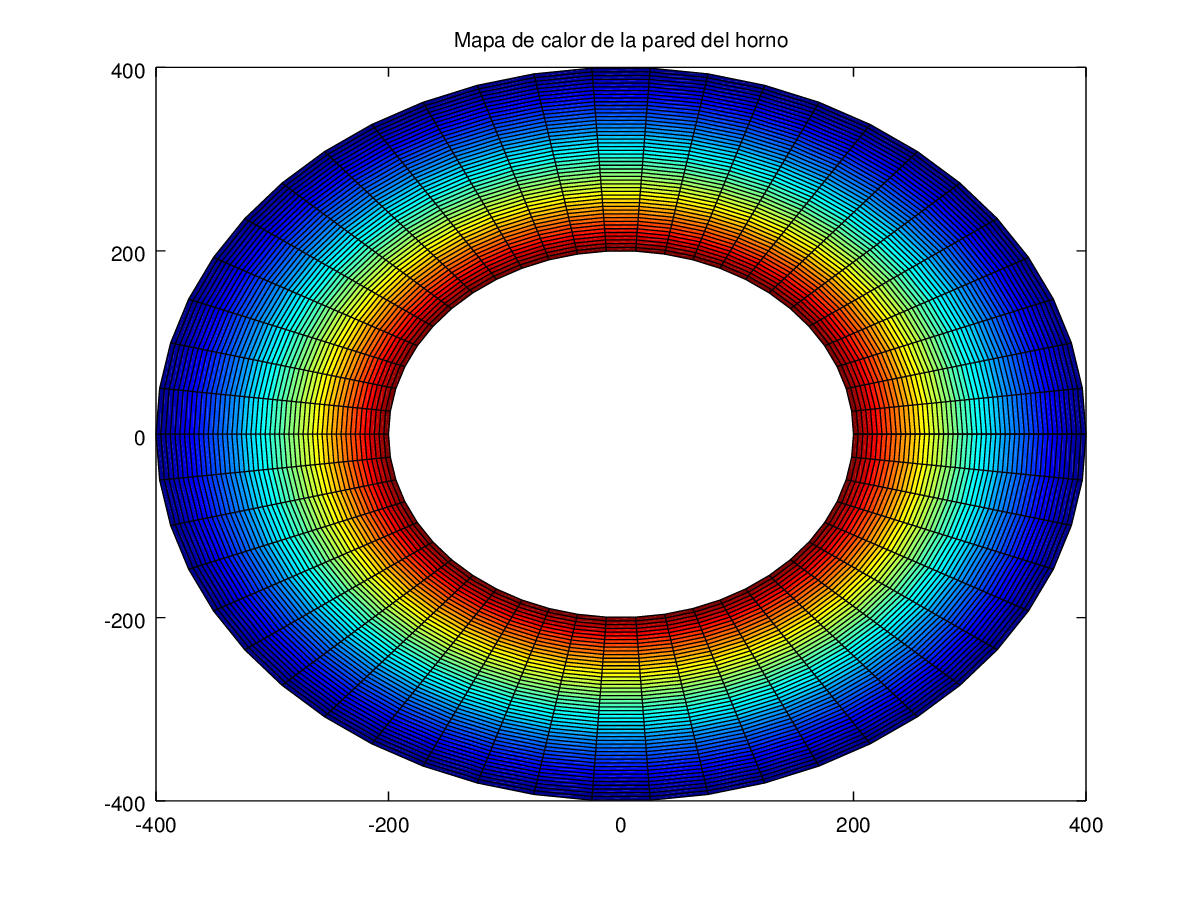
\includegraphics[scale=0.35]{experimentos1a_1b/evolucion_posicion_isoterma_temperatura/variacion_angulos_radio_fijo_se_suaviza_isoterma/test10_050_radios_050_angulos_inst_001_heatmap.png}

\vspace{0.5cm}

Aquí el radio es el mismo, pero se gana en precisión al tener más ángulos por no tener que linealizar la posición de la isoterma angularmente. Nuevamente, la posición entre dos tests consecutivos se estabiliza al aumentar la cantidad de ángulos. Tambien se observa que al cambiar el $\Delta_\theta$ los ángulos entre tests consecutivos no son los mismos.

	\item \begin{itemize}
						\item \textbf{Temperaturas internas y externas:} constantes, 100 y 1500. Esto es para que tenga la misma solución cada test del experimento.
						\item \textbf{Radio interno:} 200
						\item \textbf{Radio externo:} 400
						\item \textbf{Cantidad radios:} $[15\dots60]$
						\item \textbf{Cantidad ángulos:} $[15\dots60]$
						\item \textbf{Isoterma buscada:} 500
					\end{itemize}
	Se adjunta con el trabajo práctico un video que expone la evolución del sistema mientras se incrementa la cantidad de radios. Expondremos estáticamente algunos frames, pero es conveniente ver el video primero. Se encuentra en la misma carpeta que el pdf. (variación\_doble\_isomap.mp4, variación\_doble\_heatmap.mp4).

	\vspace{0.5cm}
	  	\textbf{Variación de la estimación de la isoterma entre 15 y 16 radios, ángulos de discretización}\\
		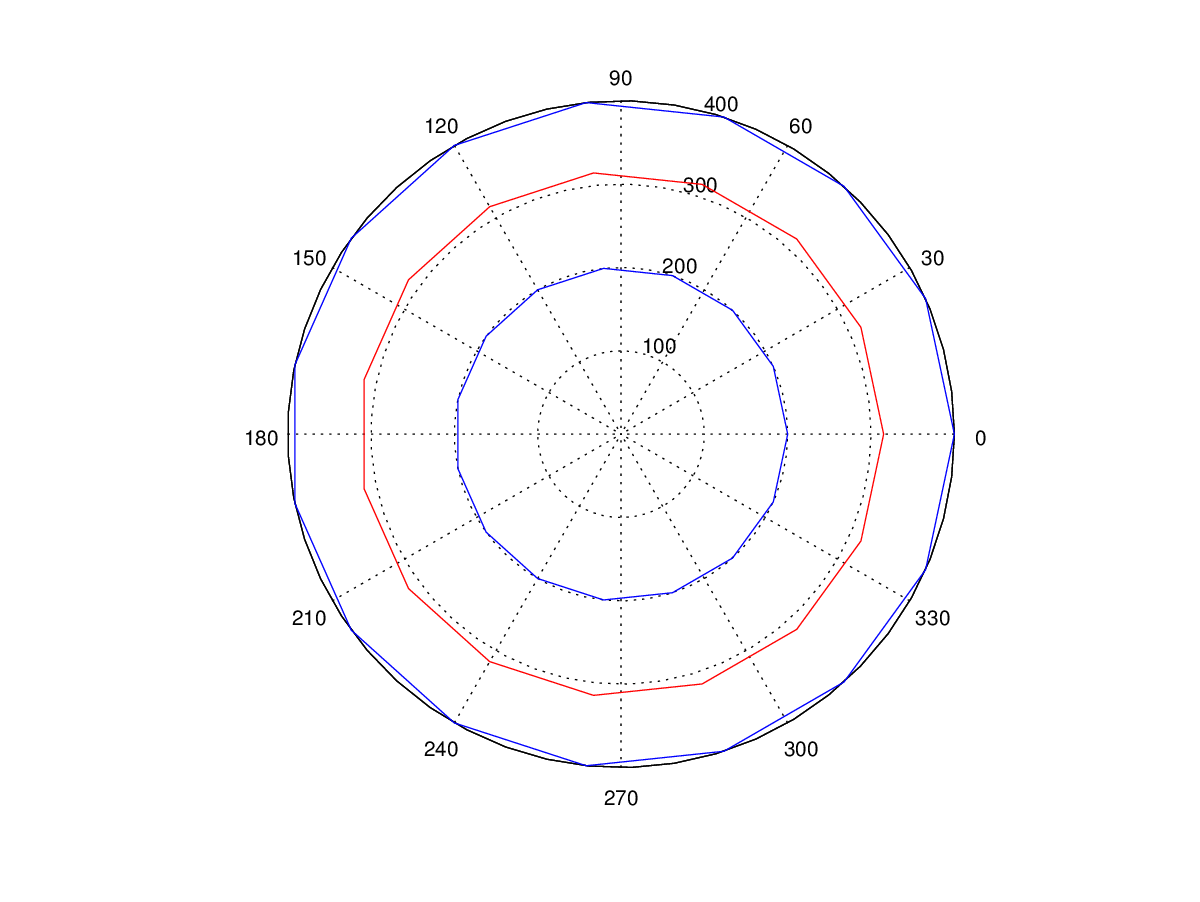
\includegraphics[scale=0.35]{experimentos1a_1b/evolucion_posicion_isoterma_temperatura/variacion_radios_angulos_se_reduce_diferencia_radial/test11_testord_001_inst_001_isomap.png}
		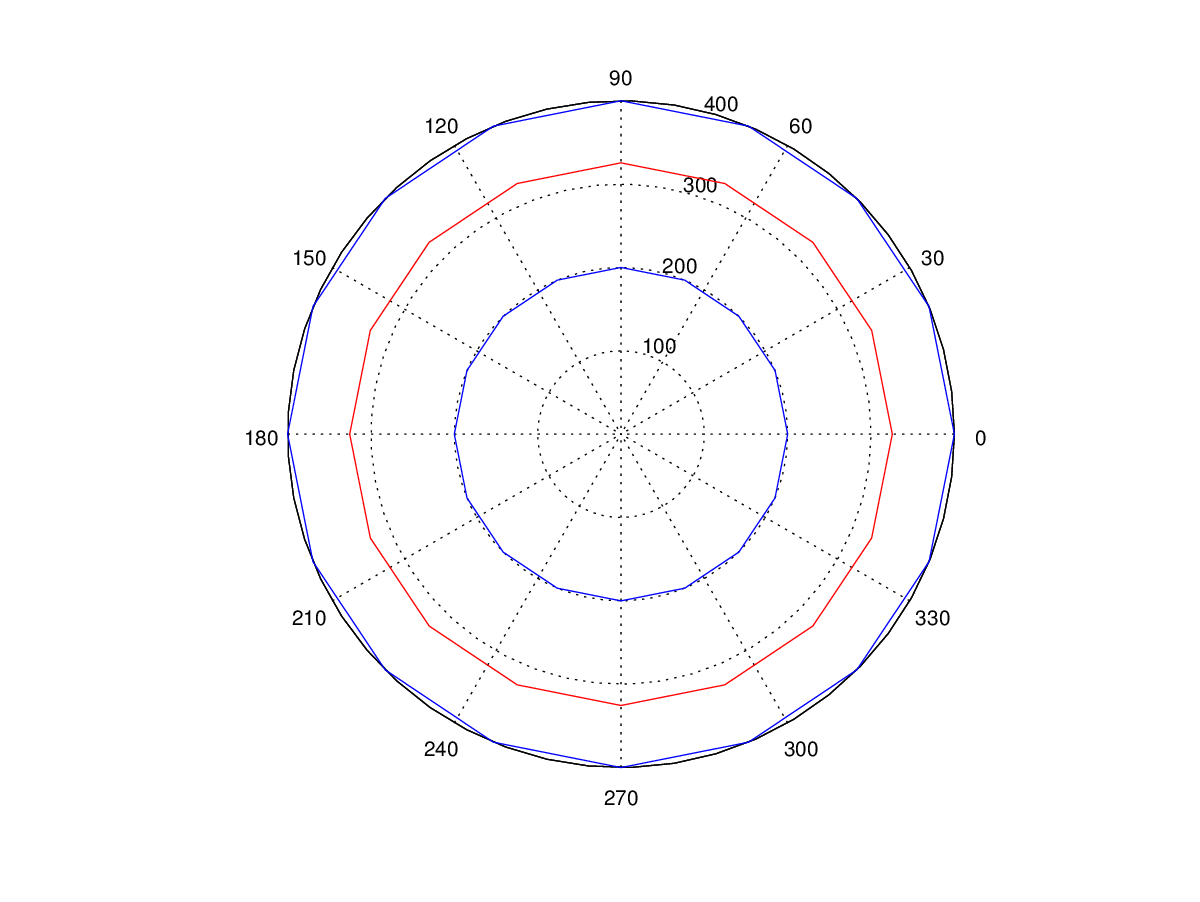
\includegraphics[scale=0.35]{experimentos1a_1b/evolucion_posicion_isoterma_temperatura/variacion_radios_angulos_se_reduce_diferencia_radial/test11_testord_002_inst_001_isomap.png}

	  	\textbf{Variación de la temperatura entre 59 y 60 radios, ángulos de discretización}\\
	  	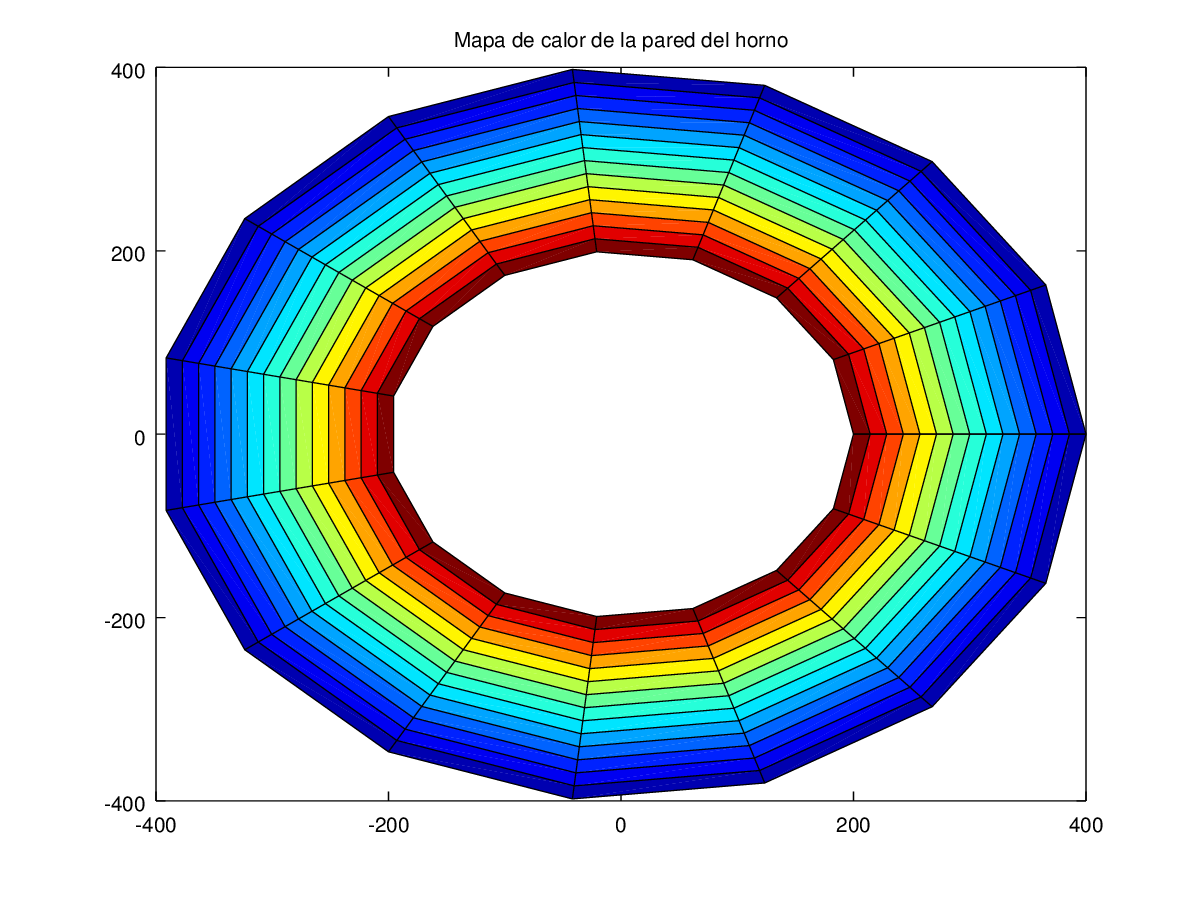
\includegraphics[scale=0.35]{experimentos1a_1b/evolucion_posicion_isoterma_temperatura/variacion_radios_angulos_se_reduce_diferencia_radial/test11_testord_001_inst_001_heatmap.png}
		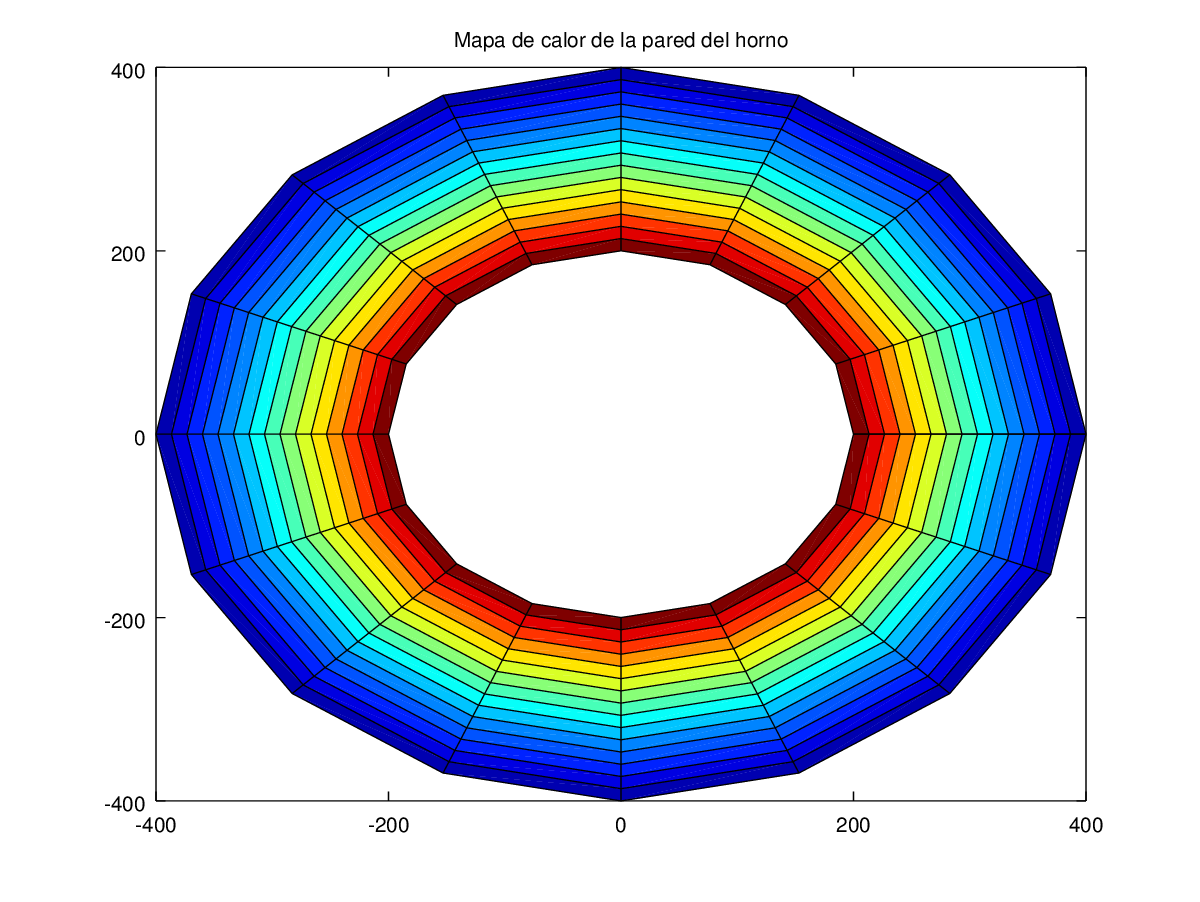
\includegraphics[scale=0.35]{experimentos1a_1b/evolucion_posicion_isoterma_temperatura/variacion_radios_angulos_se_reduce_diferencia_radial/test11_testord_002_inst_001_heatmap.png}

	  	\textbf{Variación de la estimación de la isoterma entre 15 y 16 radios, ángulos de discretización}\\
		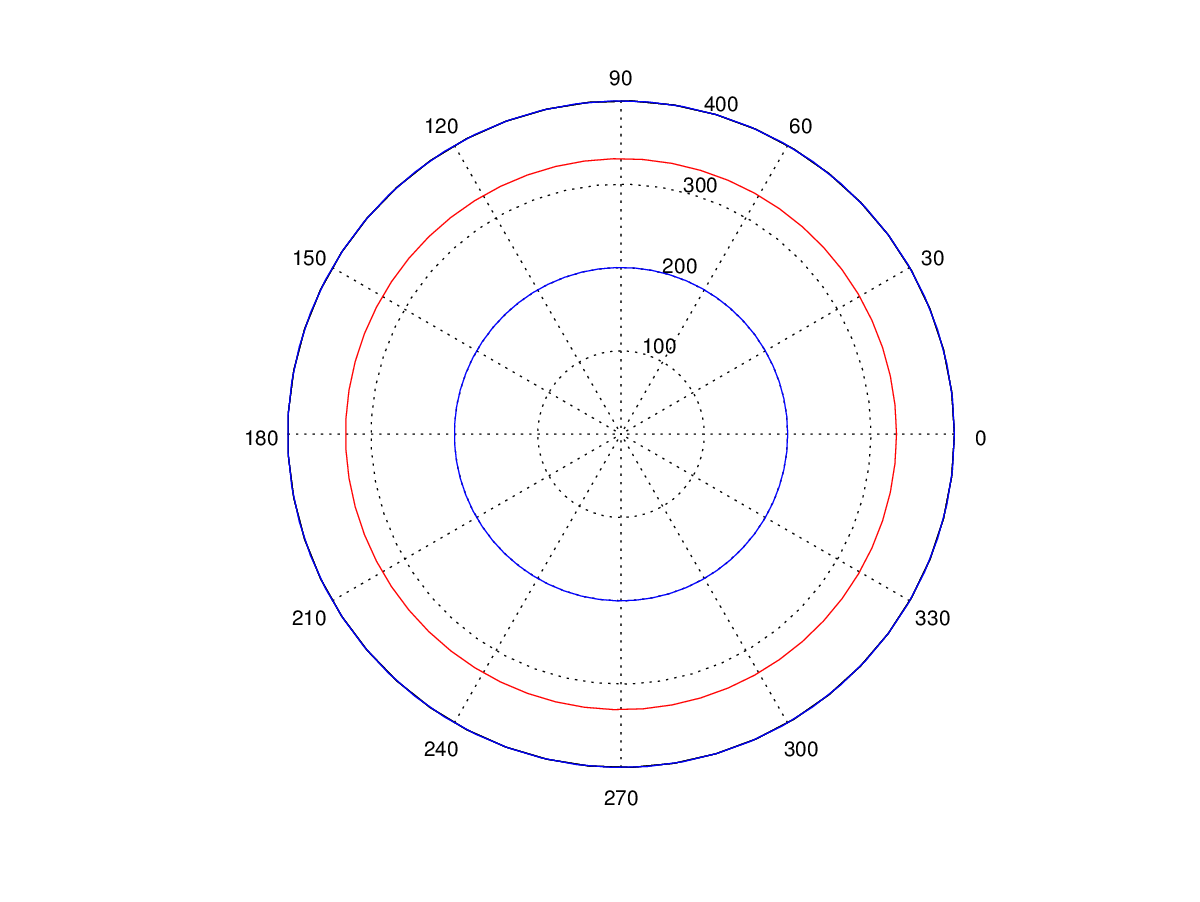
\includegraphics[scale=0.35]{experimentos1a_1b/evolucion_posicion_isoterma_temperatura/variacion_radios_angulos_se_reduce_diferencia_radial/test11_testord_045_inst_001_isomap.png}
		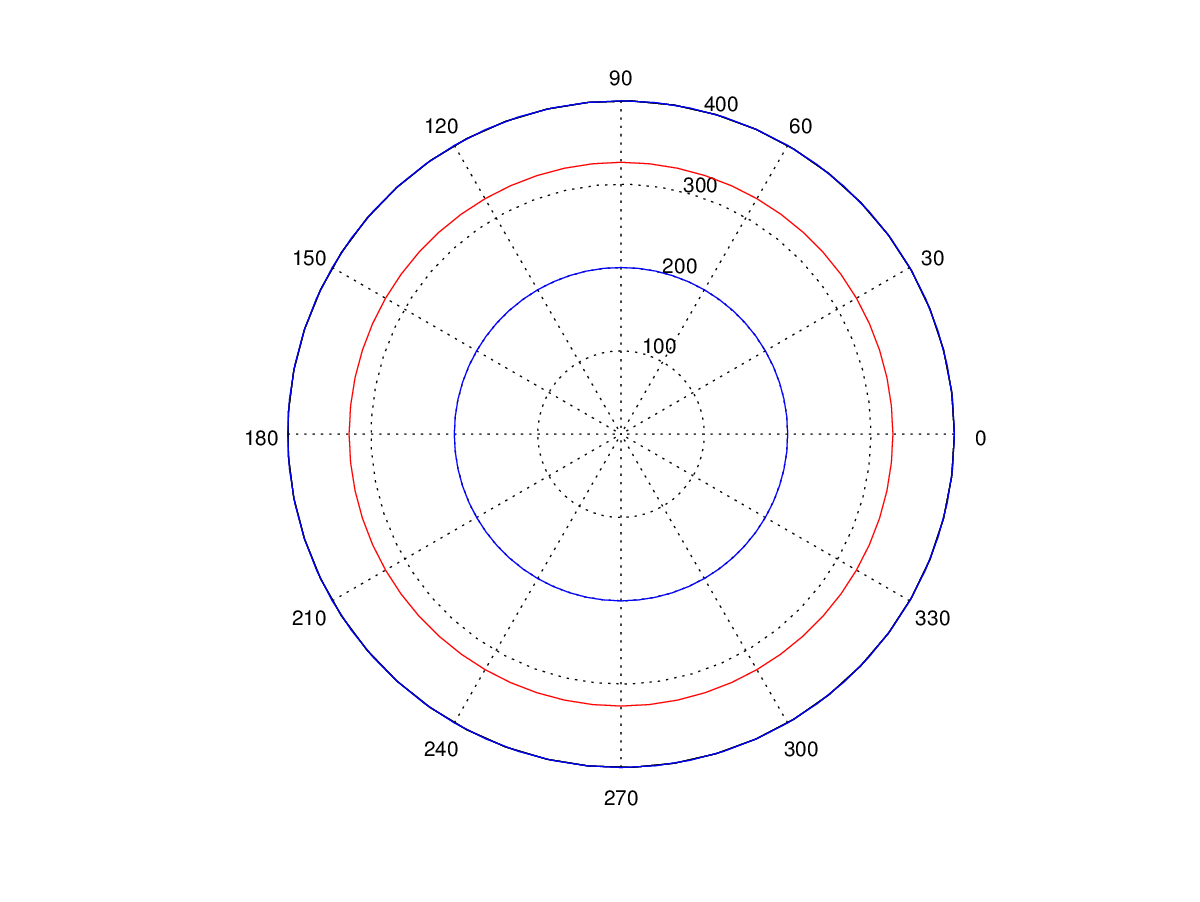
\includegraphics[scale=0.35]{experimentos1a_1b/evolucion_posicion_isoterma_temperatura/variacion_radios_angulos_se_reduce_diferencia_radial/test11_testord_046_inst_001_isomap.png}

		\textbf{Variación de la temperatura entre 59 y 60 radios, ángulos de discretización}\\
	  	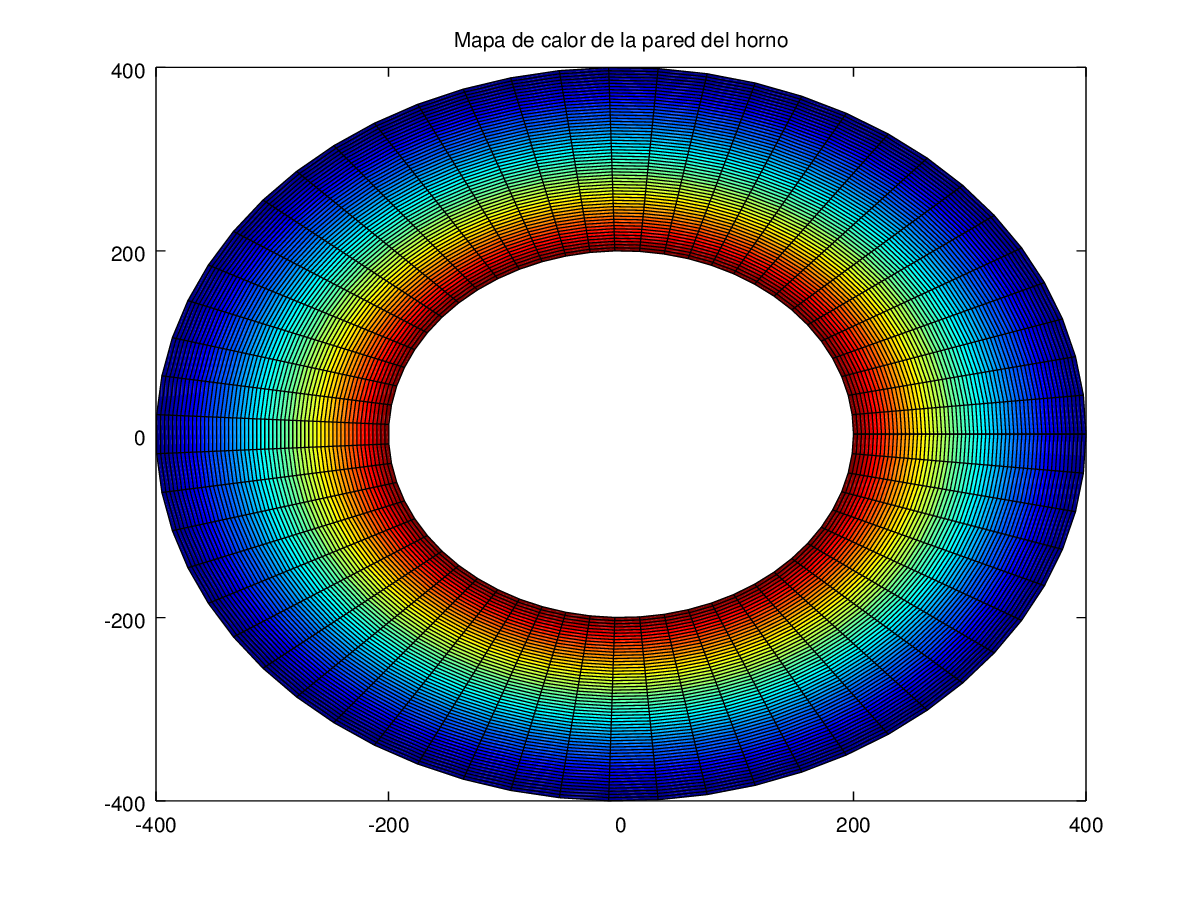
\includegraphics[scale=0.35]{experimentos1a_1b/evolucion_posicion_isoterma_temperatura/variacion_radios_angulos_se_reduce_diferencia_radial/test11_testord_045_inst_001_heatmap.png}
		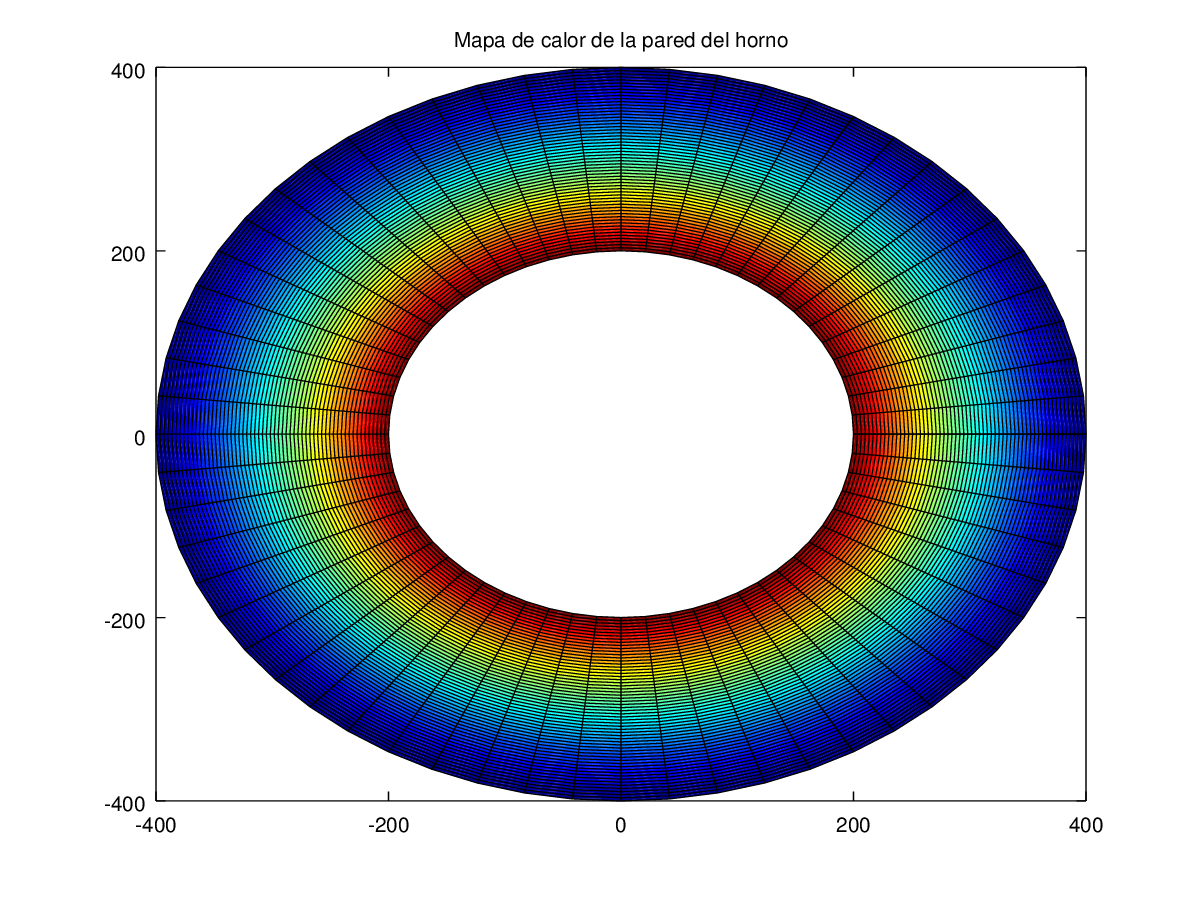
\includegraphics[scale=0.35]{experimentos1a_1b/evolucion_posicion_isoterma_temperatura/variacion_radios_angulos_se_reduce_diferencia_radial/test11_testord_046_inst_001_heatmap.png}
\FloatBarrier
\vspace{0.5cm}

En este último ejemplo ocurren ambos fenomenos al mismo tiempo, hay una variación radial menor a medida que crecen los radios y la curva se suaviza al aumentar los ángulos.

\end{enumerate}

\vspace{0.5cm}

Efectivamente, podemos concluir que mientras más fina sea la discretización, se obtendrán resultados más \texttt{estables y confiables} acerca de la estimación. Uno de los motivos es porque habrá menos puntos para interpolar en la posición de la isoterma y el otro porque se tiene más informacion de la temperatura de la pared del horno.

\subsubsection{Estimación de estabilidad de la pared del horno}

Se presentarán a continuación los resultados de la estimacion de la estabilidad del horno. Para varios tipos de discretizaciones donde la cantidad de ángulos y radios son iguales, se evalua el cambio de posicion de la isoterma a medida que va aumentando la temperatura externa entre 100 y 300 grados, de a 2 grados por paso. Dado que las temperaturas son constantes, el máximo y el promedio coinciden como métricas de posicionamiento relativo de la isoterma.

\begin{figure}[h]
\centering

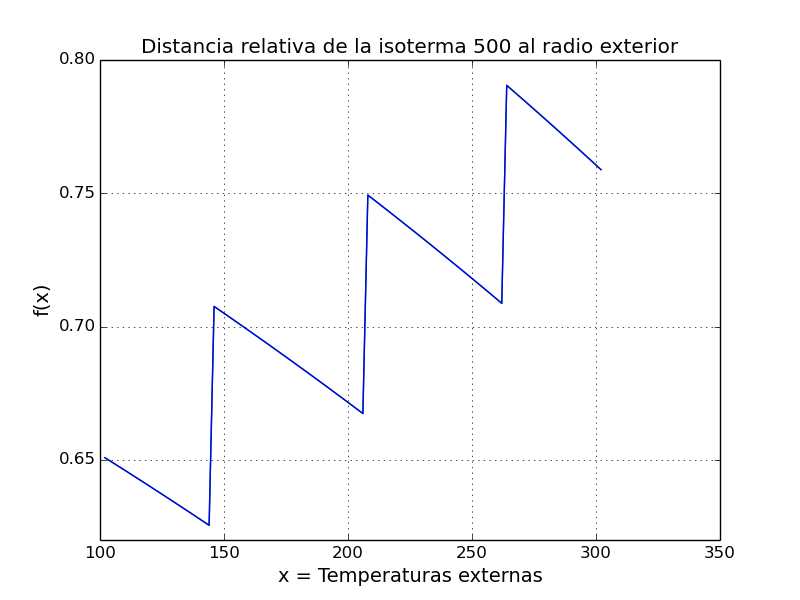
\includegraphics[scale=0.3]{experimentos1a_1b/evolucion_estimacion_seguridad_isoterma/variacion_25.png}
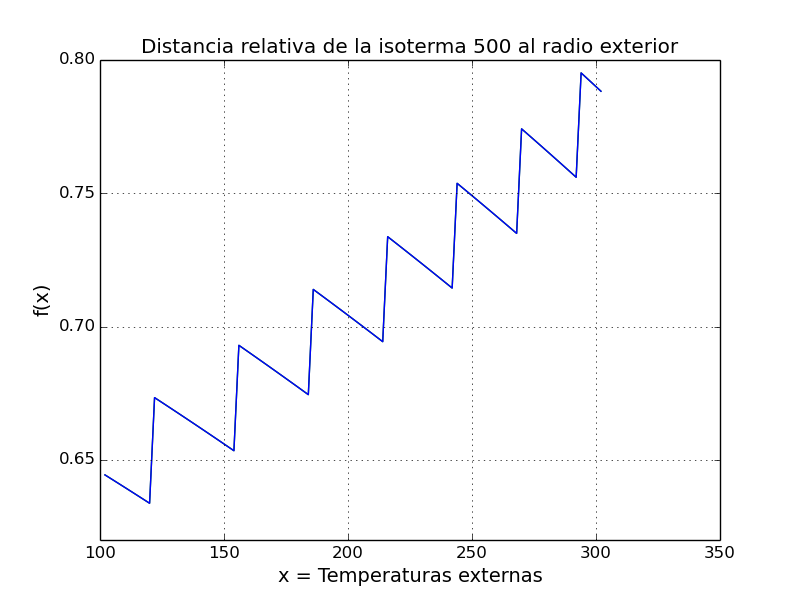
\includegraphics[scale=0.3]{experimentos1a_1b/evolucion_estimacion_seguridad_isoterma/variacion_50.png}	

\caption{Cantidad de radios y ángulos: 25(Izq) 50(Der)}
\end{figure}

\begin{figure}[h]
\centering

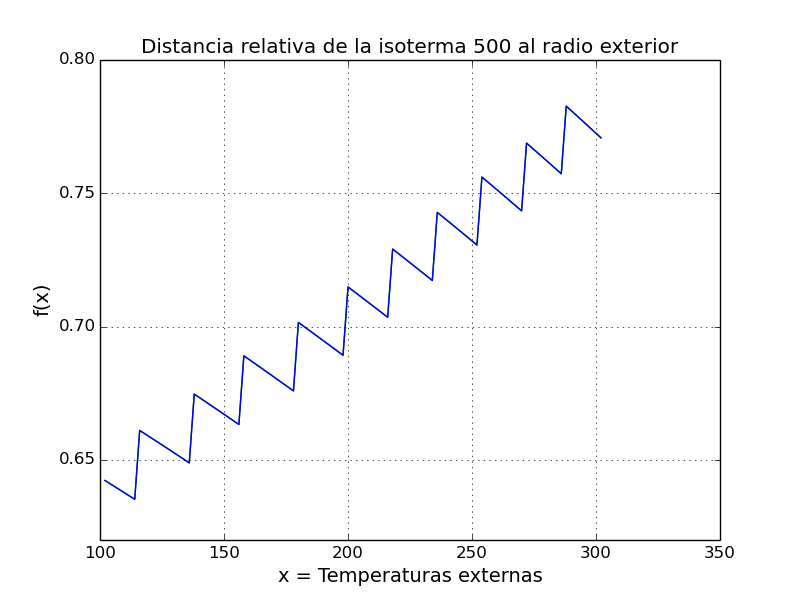
\includegraphics[scale=0.3]{experimentos1a_1b/evolucion_estimacion_seguridad_isoterma/variacion_75.png}
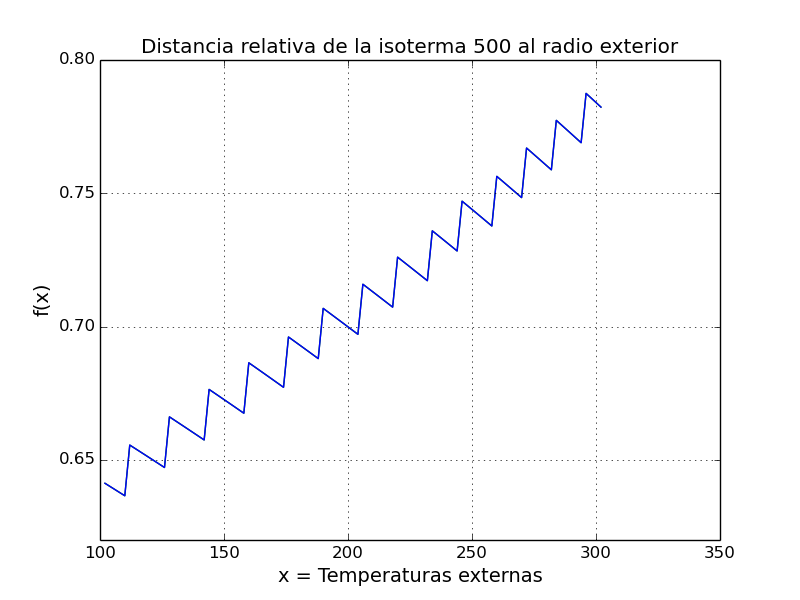
\includegraphics[scale=0.3]{experimentos1a_1b/evolucion_estimacion_seguridad_isoterma/variacion_100.png}	

\caption{Cantidad de radios y ángulos: 75(Izq) 100(Der)}
\end{figure}

\begin{figure}[h]
\centering

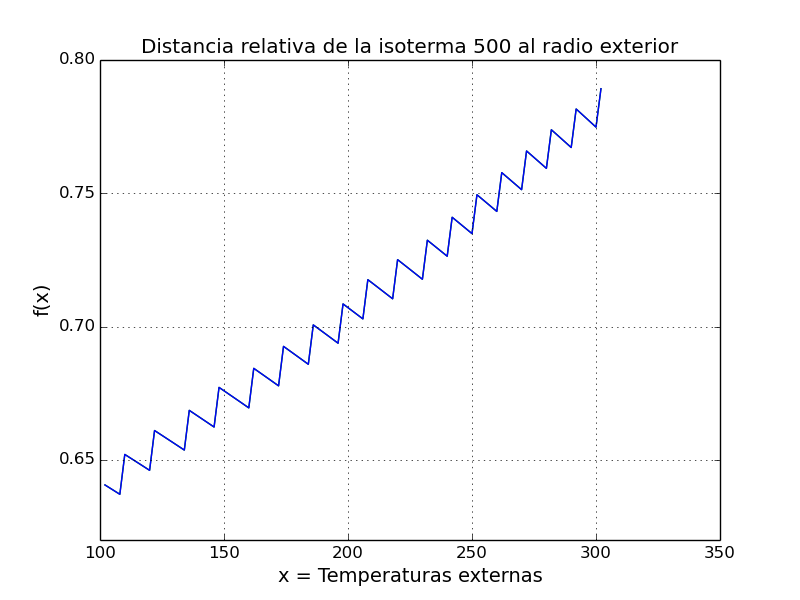
\includegraphics[scale=0.5]{experimentos1a_1b/evolucion_estimacion_seguridad_isoterma/variacion_125.png}

\caption{Cantidad de radios y ángulos: 125}
\end{figure}

\begin{figure}[h]
\centering

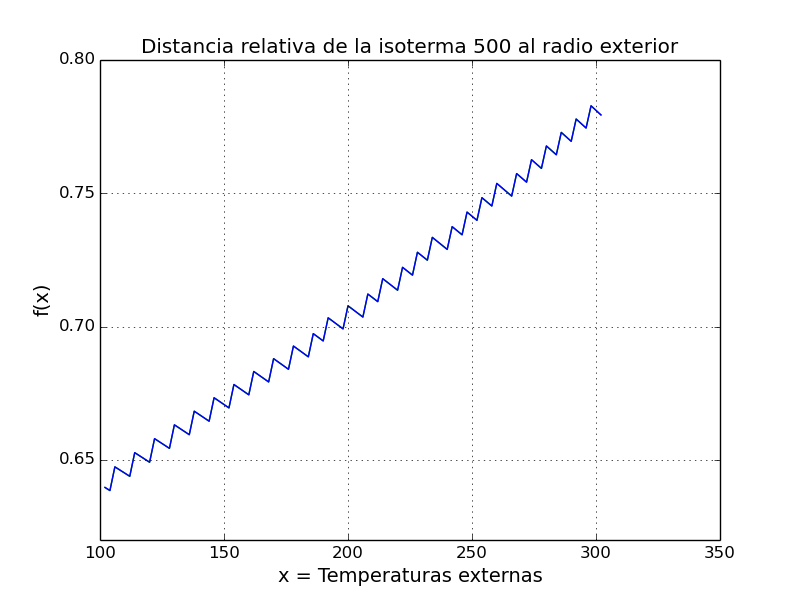
\includegraphics[scale=0.5]{experimentos1a_1b/evolucion_estimacion_seguridad_isoterma/variacion_30a_200r.png}
\caption{Cantidad de radios 200 - ángulos: 30}

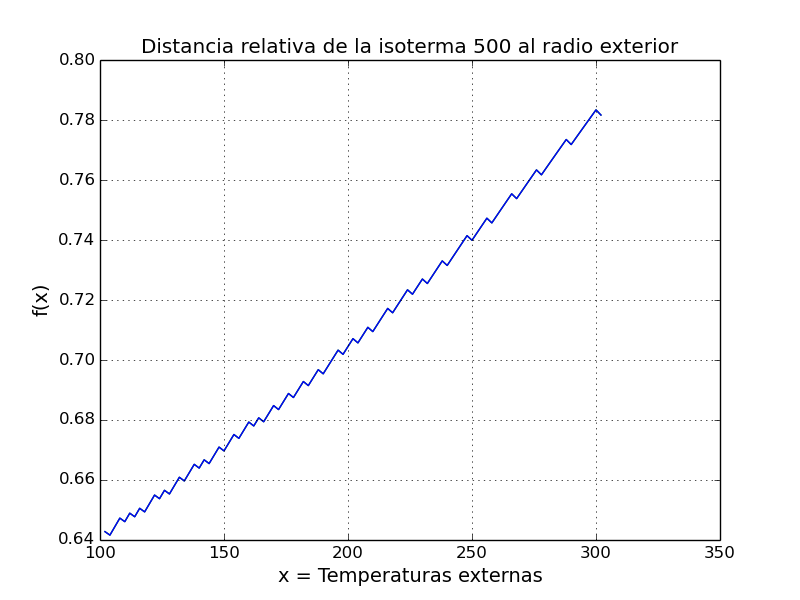
\includegraphics[scale=0.5]{experimentos1a_1b/evolucion_estimacion_seguridad_isoterma/variacion_5a_500r.png}
\caption{Cantidad de radios 500 - ángulos: 5}
\end{figure}
\FloatBarrier

Los gráficos son un poco mas extraños de lo esperado. Se observa que, para cualquier discretizacion fija, al aumentar la temperatura externa, la isoterma tiende a acercarse a la pared externa. Esto es lo esperable, el método propuesto para determinar la seguridad de la isoterma consiste en fijar un umbral sobre la posicion relativa máxima o promedio. Lo que se observa como raro es la curva \texttt{dentada} a medida que crecen las temperaturas. Veamos además que estos \texttt{dientes} disminuyen su intensidad a medida que se van agregando radios a la discretizacion. 

\begin{proposition} 
	Bajo que las temperaturas internas y externas constantes, la posicion radial de la isoterma es la misma en todo ángulo.	
\end{proposition}

Dada esta última proposición, podemos hacer experimentos con muy pocos ángulos y muchos radios que nos den pauta de que ocurre con esos \texttt{dientes} en los gráficos. \\
Se puede observar en las figuras con 200 y 500 radios, que a medida que $m\to\infty$ , la curva se suaviza. Lo cual nos hace pensar, que la estimacion lineal de la isoterma esta generando esta distorsión.

\vspace{0.5cm}

Consideremos nuevamente $\hat{g_{\theta_i}}$: la función \textbf{discreta de aproximaciones} de temperatura de un ángulo i. A medida que las temperaturas aumentan linealmente, los 2 puntos $x$ y $x'$ que acotan la isoterma buscada en dicha función van aumentando tambien, generando que la estimacion del punto intermedio entre ellos decrezca. Creemos que cuando esos 2 puntos dejan se encerrar el valor buscado, es que se produce el \texttt{salto} en el gráfico.

\begin{proposition}
	El método de umbral de seguridad es inconsistente tomando la distancia máxima relativa o distancia promedio relativa a la pared exterior.
\end{proposition}

En los resultados anteriores y en el gráfico presentado en el primer experimento de ubicacion de la isoterma (convergencia radial de la isoterma). Se puede observar claramente, que trazando una recta horizontal en algún punto del eje Y, la determinación de colapso no es consistente. Es decir, existen $t_1 < t_2 < t_3$ temperaturas crecientes donde tanto la posicion máxima relativa o la posicion promedio relativa, indican peligro de colapso para $t_2$ pero no para $t_1$ ni $t_3$. Sin embargo, cuando $m\to\infty$ esto tiende a ser \texttt{menos inconsistente}.

\subsubsection{Análisis de la interpolacion lineal de la curva de temperatura}

Dados los resultados de la sección anterior, nos interesó saber un poco mas la forma de la funcion de temperatura sobre un ángulo fijo $\hat{g_{\theta_i}}$. 
Variamos un poco la cantidad de radios, y graficamos la función obtenida de los puntos de la discretización en una dirección fija y un fitteo lineal.
El resultado de los gráficos muestra que la temperatura no se disipa linealmente entre el interior y el exterior del horno. Dado que nosotros aproximamos linealmente la posicion radial de la isoterma 500 \textbf{entre los 2 puntos mas cercanos}, tendremos un error en cada \texttt{cambio de puntos} para la aproximacion.\\

Esto fortalece nuestra hipótesis de la sección anterior de que la forma de diente de sierra de los gráficos podía deberse a la interpolacion de algo no lineal, mediante una recta en puntos consecutivos.

\begin{figure}[h]
\centering
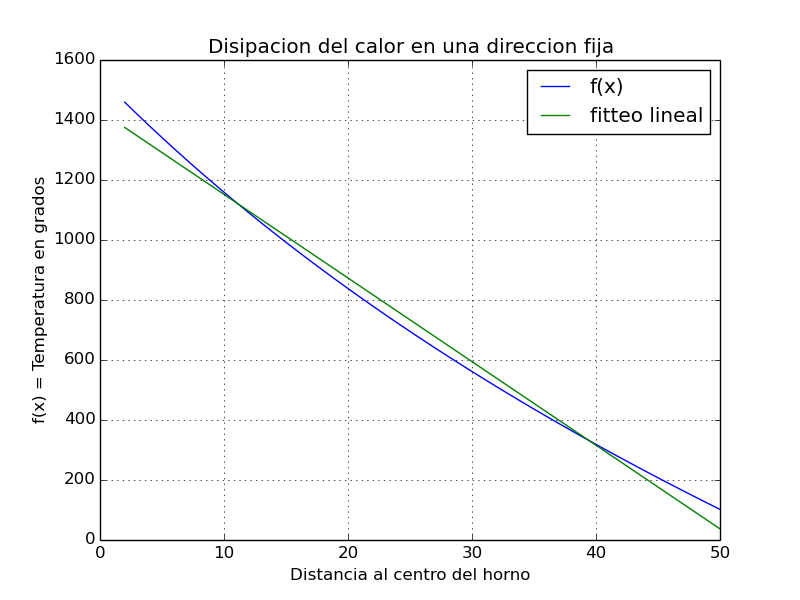
\includegraphics[scale=0.34]{funcion_temp_50_radios_ti_1500_te_102.png}
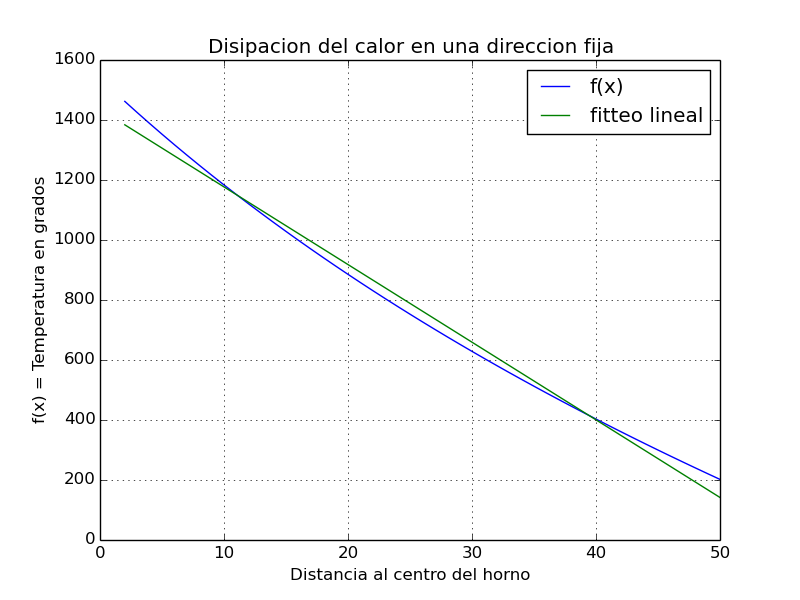
\includegraphics[scale=0.34]{funcion_temp_50_radios_ti_1500_te_202.png}
\caption{Distintas temperaturas externas - Cantidad de radios: 50}
\end{figure}
\FloatBarrier

\begin{figure}[h]
\centering
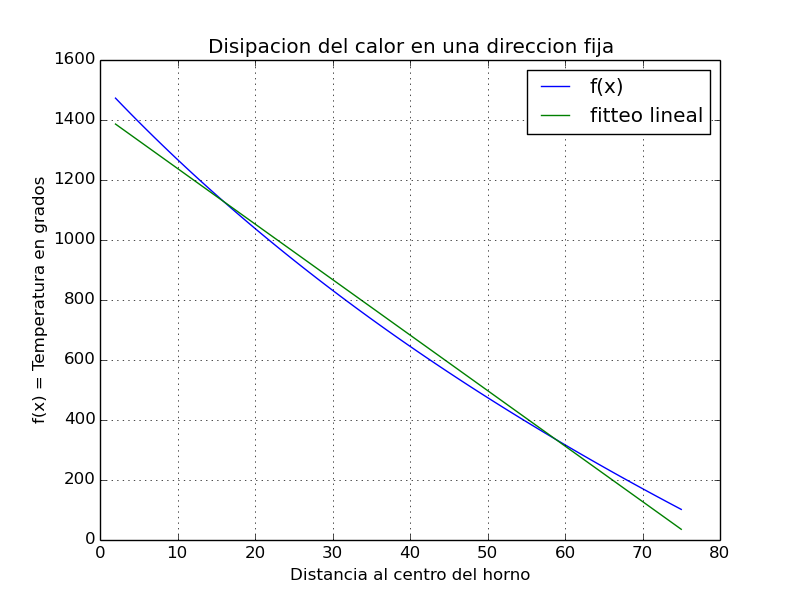
\includegraphics[scale=0.34]{funcion_temp_75_radios_ti_1500_te_102.png}
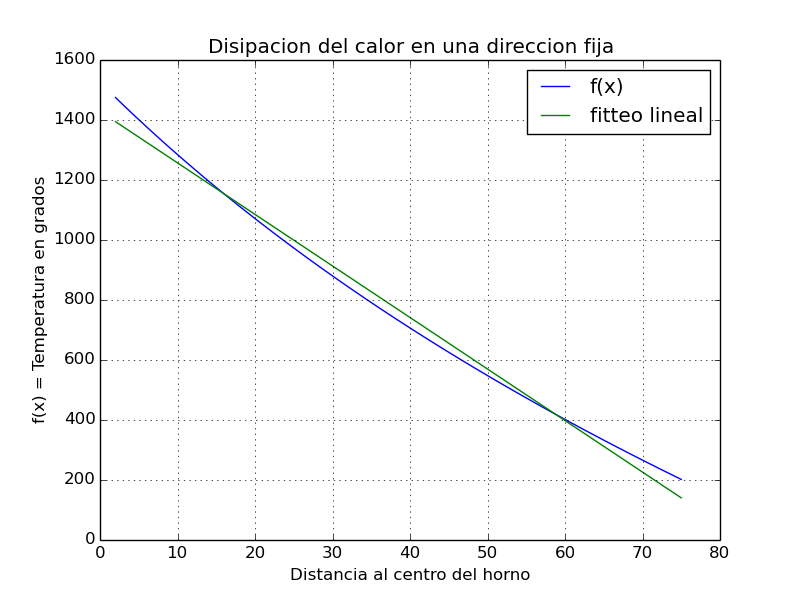
\includegraphics[scale=0.34]{funcion_temp_75_radios_ti_1500_te_202.png}
\caption{Distintas temperaturas externas - Cantidad de radios: 75}
\end{figure}
\FloatBarrier

\begin{figure}[h]
\centering
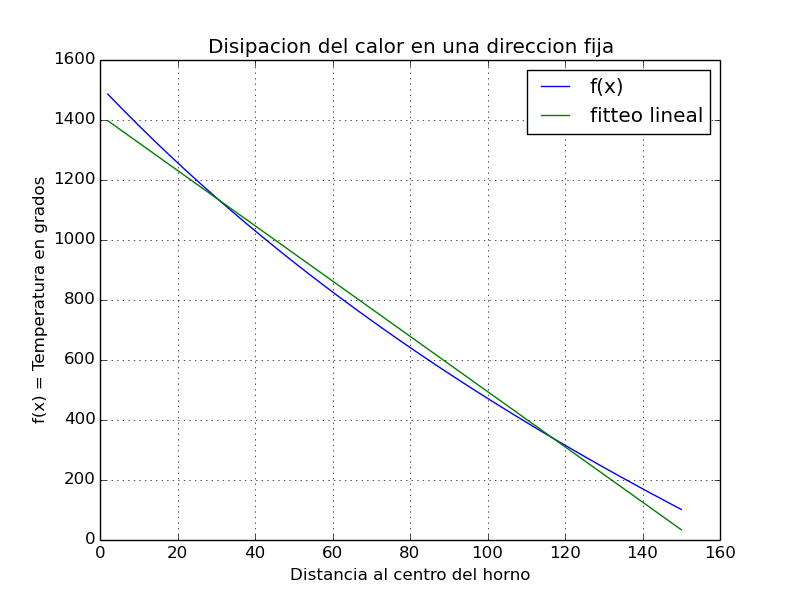
\includegraphics[scale=0.34]{funcion_temp_150_radios_ti_1500_te_102.png}
\includegraphics[scale=0.34]{funcion_temp_500_radios_ti_1500_te_102.png}
\caption{Cantidad de radios: 150(izq) , 500(der)}
\end{figure}
\FloatBarrier

\begin{figure}[h]\label{aprox}
\centering
\includegraphics[scale=0.8]{efecto_interpolacion_lineal.png}
\caption{Esquema aproximado: Efecto interpolacion lineal entre puntos de algo no lineal}
\end{figure}
\FloatBarrier

En la figura se ve lo que podría estar ocurriendo al aproximar linealmente 2 puntos de una curva que realmente no es lineal. La recta entre dos puntos queda por encima de la curva real, luego, si se quiere hallar el $x$ tal que $g(x) = \alpha$ , la aproximación falla por un $\epsilon$ que depende de la concavidad de la curva respecto a la recta. A medida que se van agregando radios a la discretizacion, la distancia entre los puntos que se aproximan disminuye, disminuyendo el error cometido al estimar. 

